\chapter{Part III(a) - Memory Hierarchy - Virtual Memory - W.7.2}
\section{Segmentation Fault: Understanding the Cause}

Segmentation faults occur when a program attempts to access a memory location that is either invalid or restricted. Consider the following C code snippet:

\begin{center}
    \begin{tikzpicture}
        \node[rounded corners=30pt, draw=none] {\includegraphics[width=0.65\textwidth]{chapters/chapter3c/images/terminal.png}};
    \end{tikzpicture}
\end{center}

In this example:
\begin{itemize}
    \item The pointer \texttt{p} is assigned the value \texttt{1234}, which is an arbitrary and invalid memory address.
    \item When the program attempts to dereference \texttt{p} using \texttt{*p} to access the value at memory address \texttt{1234}, it triggers a segmentation fault because the program does not have permission to access this memory.
\end{itemize}

\textbf{Why This Happens:}
\begin{itemize}
    \item Modern operating systems enforce memory protection, disallowing access to memory that the program does not explicitly allocate or own.
    \item Hardcoding arbitrary addresses, like \texttt{1234}, is unsafe and violates these protections.
\end{itemize}

\textbf{Assembly Analysis:}
The following assembly instructions illustrate how the invalid memory access occurs:
\begin{itemize}
    \item \texttt{li t0, 1234} -- Load the immediate value \texttt{1234} into register \texttt{t0}.
    \item \texttt{lw a1, 0(t0)} -- Attempt to load a word from address \texttt{1234}.
    \item This results in a segmentation fault because address \texttt{1234} is not valid or accessible.
\end{itemize}

We need to be able to protect memory and prevent such invalid accesses. This is where memory protection mechanisms come into play.

\subsection{Overview - Problems to Solve}
Three main problems need to be addressed:

\begin{enumerate}
    \item \textbf{Memory Protection:} How can we protect memory so that each program (or process) running simultaneously in the system can only access its own data? How can processes be isolated from each other?
    \item \textbf{Insufficient Main Memory:} What happens if the main memory (DRAM) is not sufficient for the execution of a program? Can we utilize the disk to address this limitation? If so, how?
    \item \textbf{Running Multiple Programs:} How can we run several programs (processes) simultaneously? How can multiple programs be loaded into memory efficiently, and where should they be stored?
\end{enumerate}

\section{Relocation at Load Time}

Relocation at load time is a fundamental memory management process that adjusts memory addresses to align a program’s instructions with the actual memory layout during execution. This technique ensures that all address references within the program are accurate, allowing it to run seamlessly in its allocated memory space.

\textbf{Address Adjustments:} During the relocation process, address references within instructions are updated from placeholder values (e.g., \texttt{0x0000}) to their correct memory addresses (e.g., \texttt{0x1270} or \texttt{0x1248}). This adjustment applies to all memory references, including branches and jumps such as \texttt{beq} or \texttt{j}, which depend on accurate target addresses to function correctly.
\begin{center}
    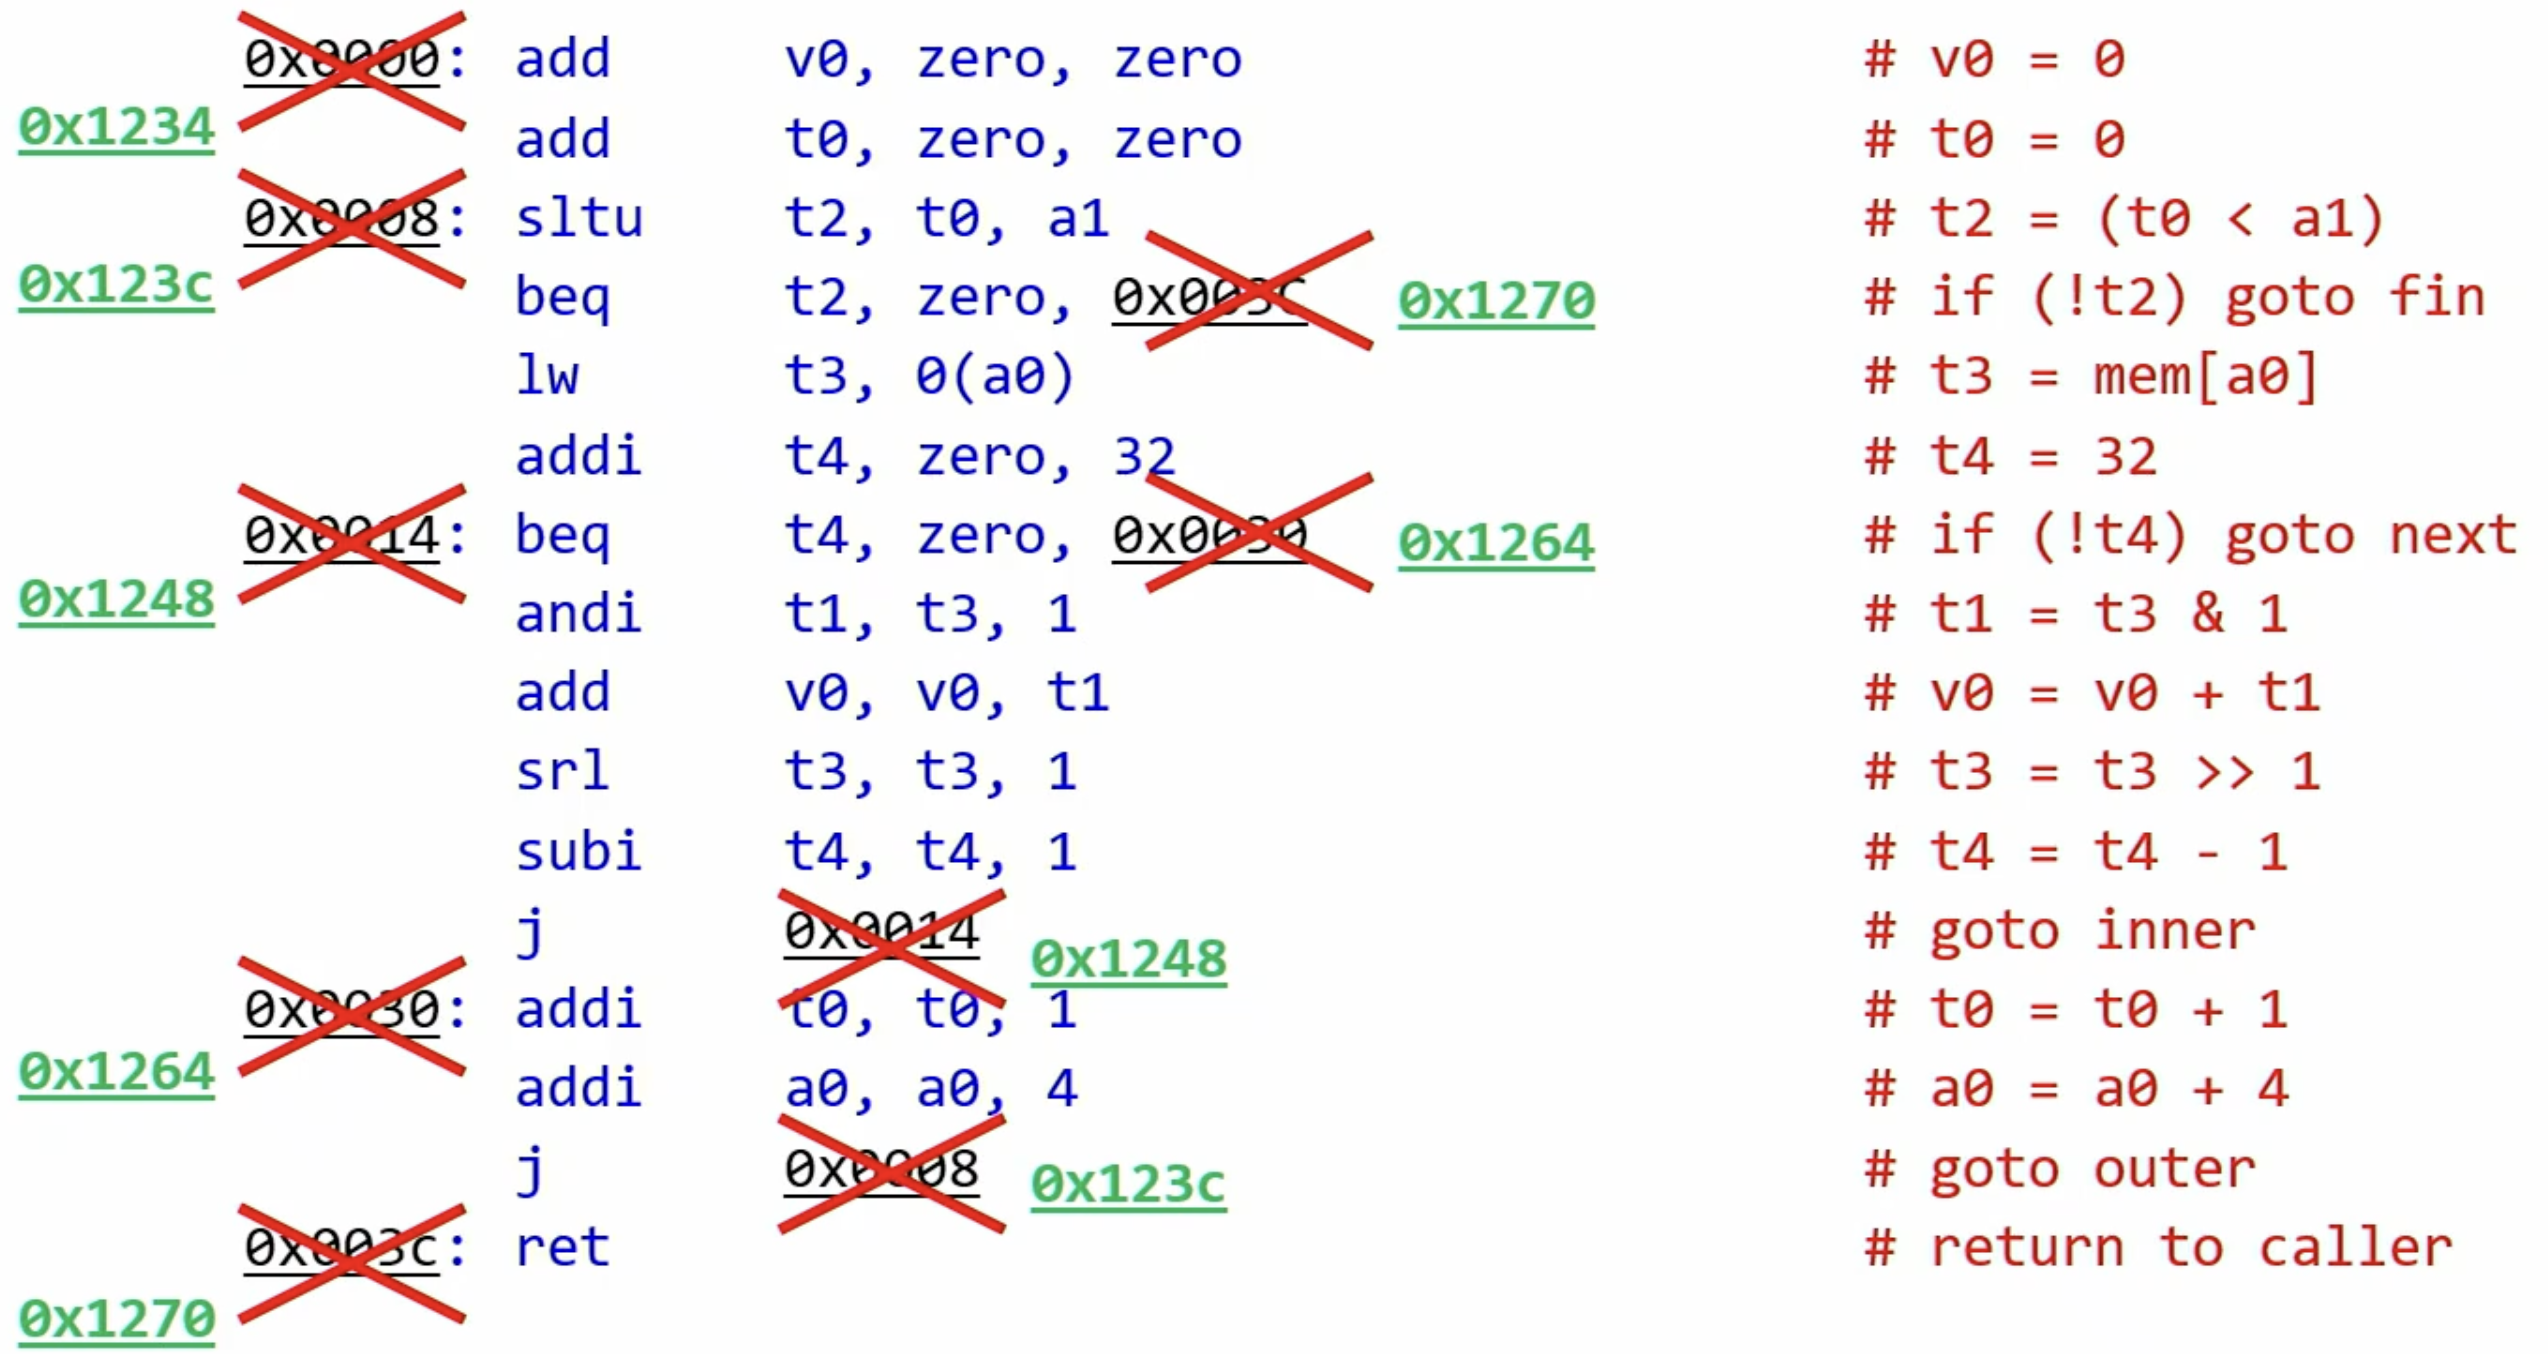
\includegraphics[width=0.65\textwidth]{chapters/chapter3c/images/relocate.png}
\end{center}

By performing these updates, the program adapts to the memory layout without requiring additional runtime computations. This process, though effective, operates primarily at the binary level rather than at the assembly code level.

\subsubsection{Binary-Level Adjustments}

Relocation at load time involves modifying the binary code directly. Specific fields within the machine instructions are updated based on relocation tables, which specify the exact memory addresses to be adjusted. These tables play a crucial role in streamlining the relocation process and ensuring correctness.
\begin{center}
    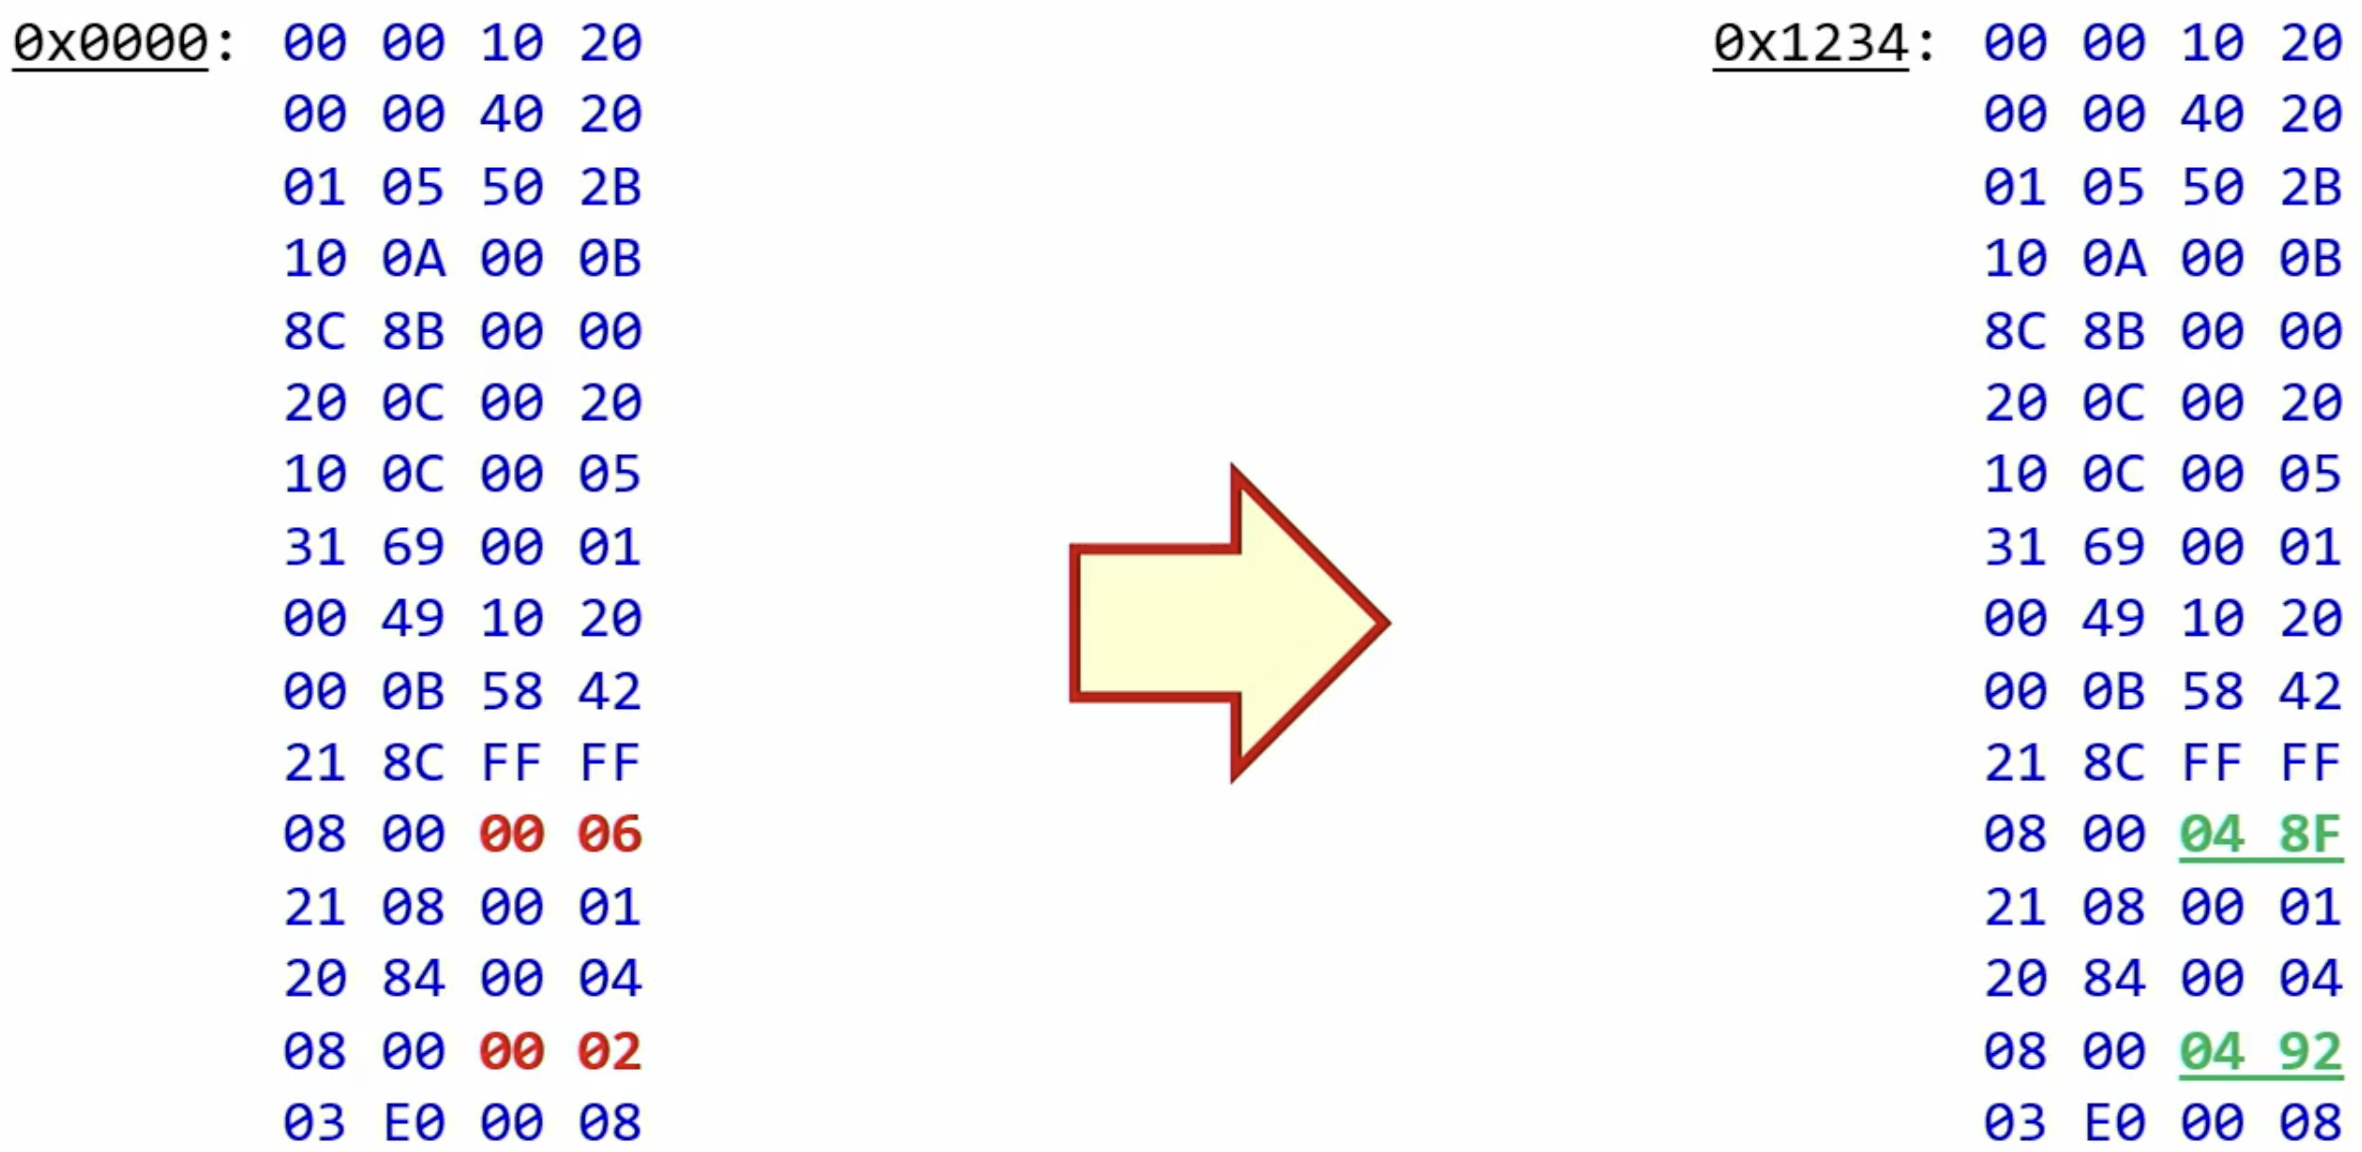
\includegraphics[width=0.65\textwidth]{chapters/chapter3c/images/relocate2.png}
\end{center}

For instance, consider a binary program initially loaded at a base address of \texttt{0x0000}. During relocation, placeholders in the binary instructions are replaced with actual memory addresses derived from the relocation table, as illustrated in the figure. This guarantees that memory references resolve correctly during execution.

\subsubsection{Memory Utilization and Limitations}

While relocation at load time simplifies memory address management, it is not without its drawbacks. As programs are loaded and terminated, gaps in memory may form, leading to inefficient utilization. This fragmentation becomes particularly problematic in systems with limited memory or dynamic memory allocation needs.
\begin{center}
    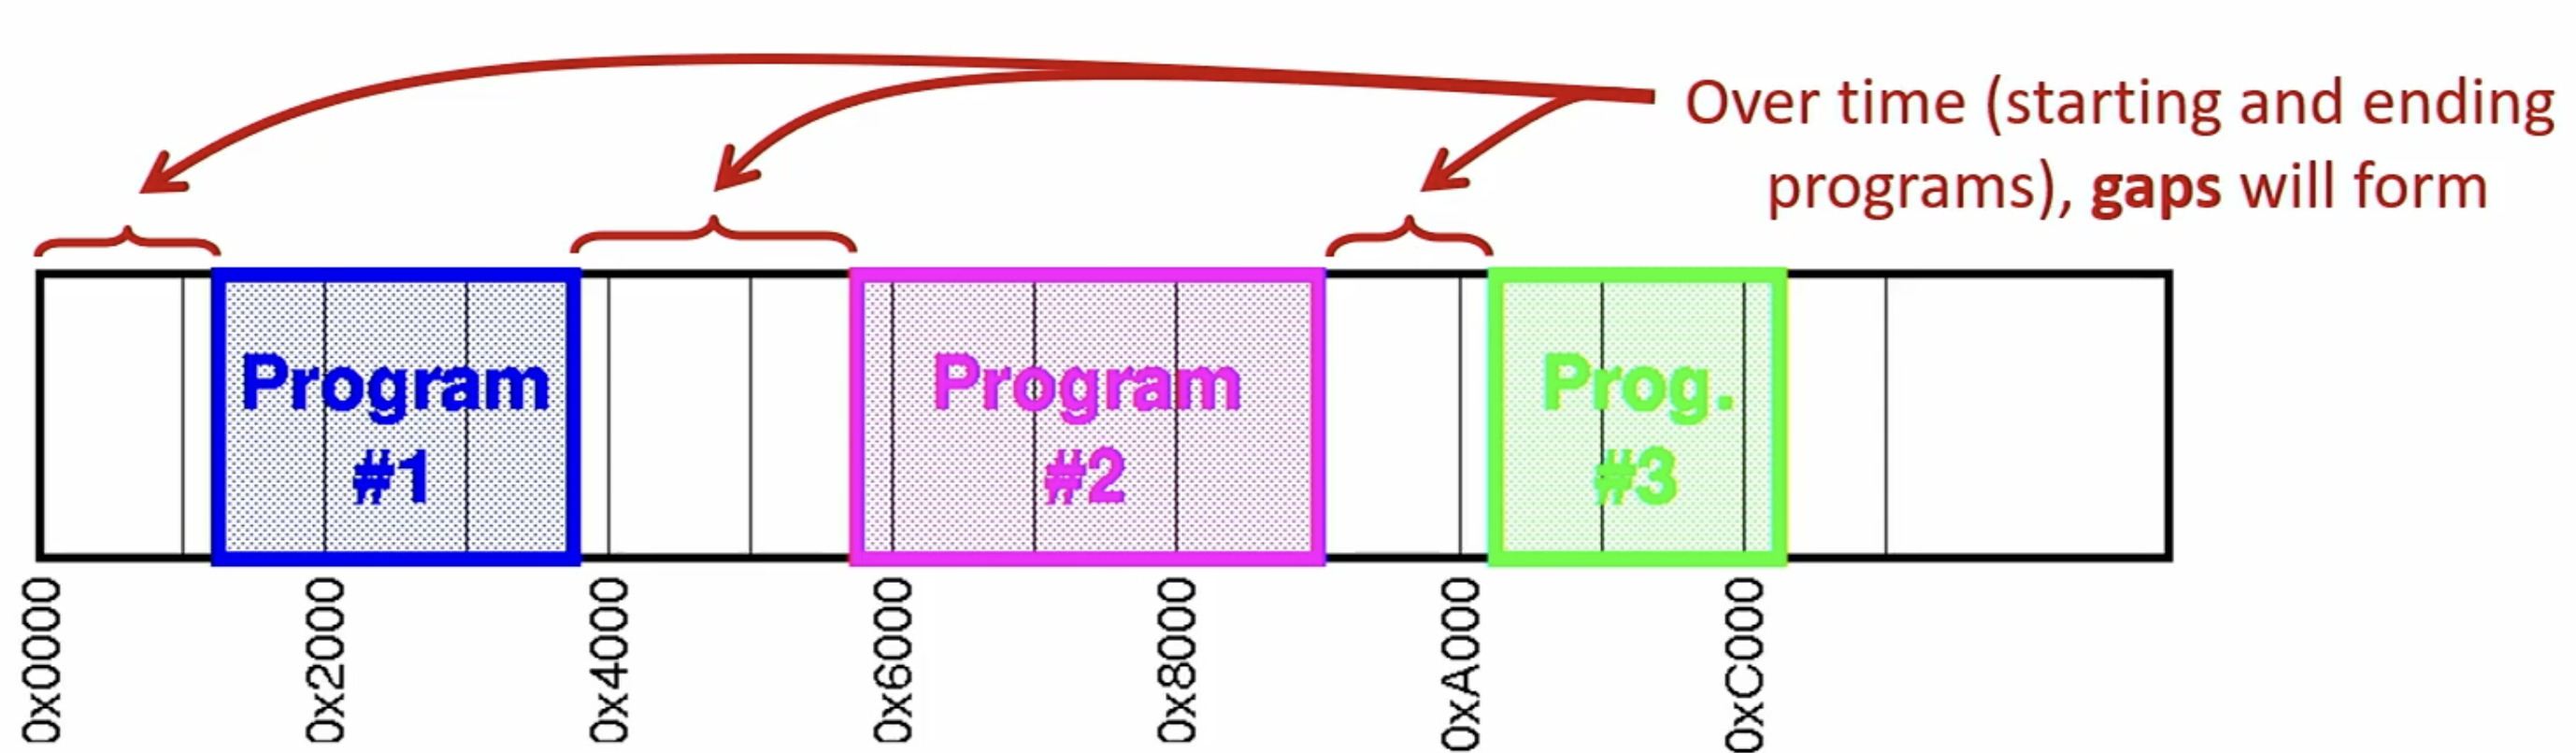
\includegraphics[width=0.65\textwidth]{chapters/chapter3c/images/relocate3.png}
\end{center}

\textbf{Limitations:}
\begin{itemize}
    \item \textit{High Overhead:} Relocation requires considerable computational effort at load time to allocate and adjust memory segments accurately.
    \item \textit{Inflexibility:} Once memory is allocated, it cannot be dynamically reconfigured, making it challenging to adapt to changing program requirements.
    \item \textit{Fragmentation Constraints:} Memory fragmentation caused by terminated programs can prevent loading a new program if its size exceeds the largest available gap, even when total free memory is sufficient (garbage collector\dots).
\end{itemize}
\subsection{Relocation in Hardware: Base and Bounds MMU}
Memory relocation is an essential process in modern computer systems to map virtual addresses to physical addresses. The \textbf{Base and Bounds Memory Management Unit (MMU)} facilitates this process dynamically by ensuring secure and efficient address translation.
\begin{center}
    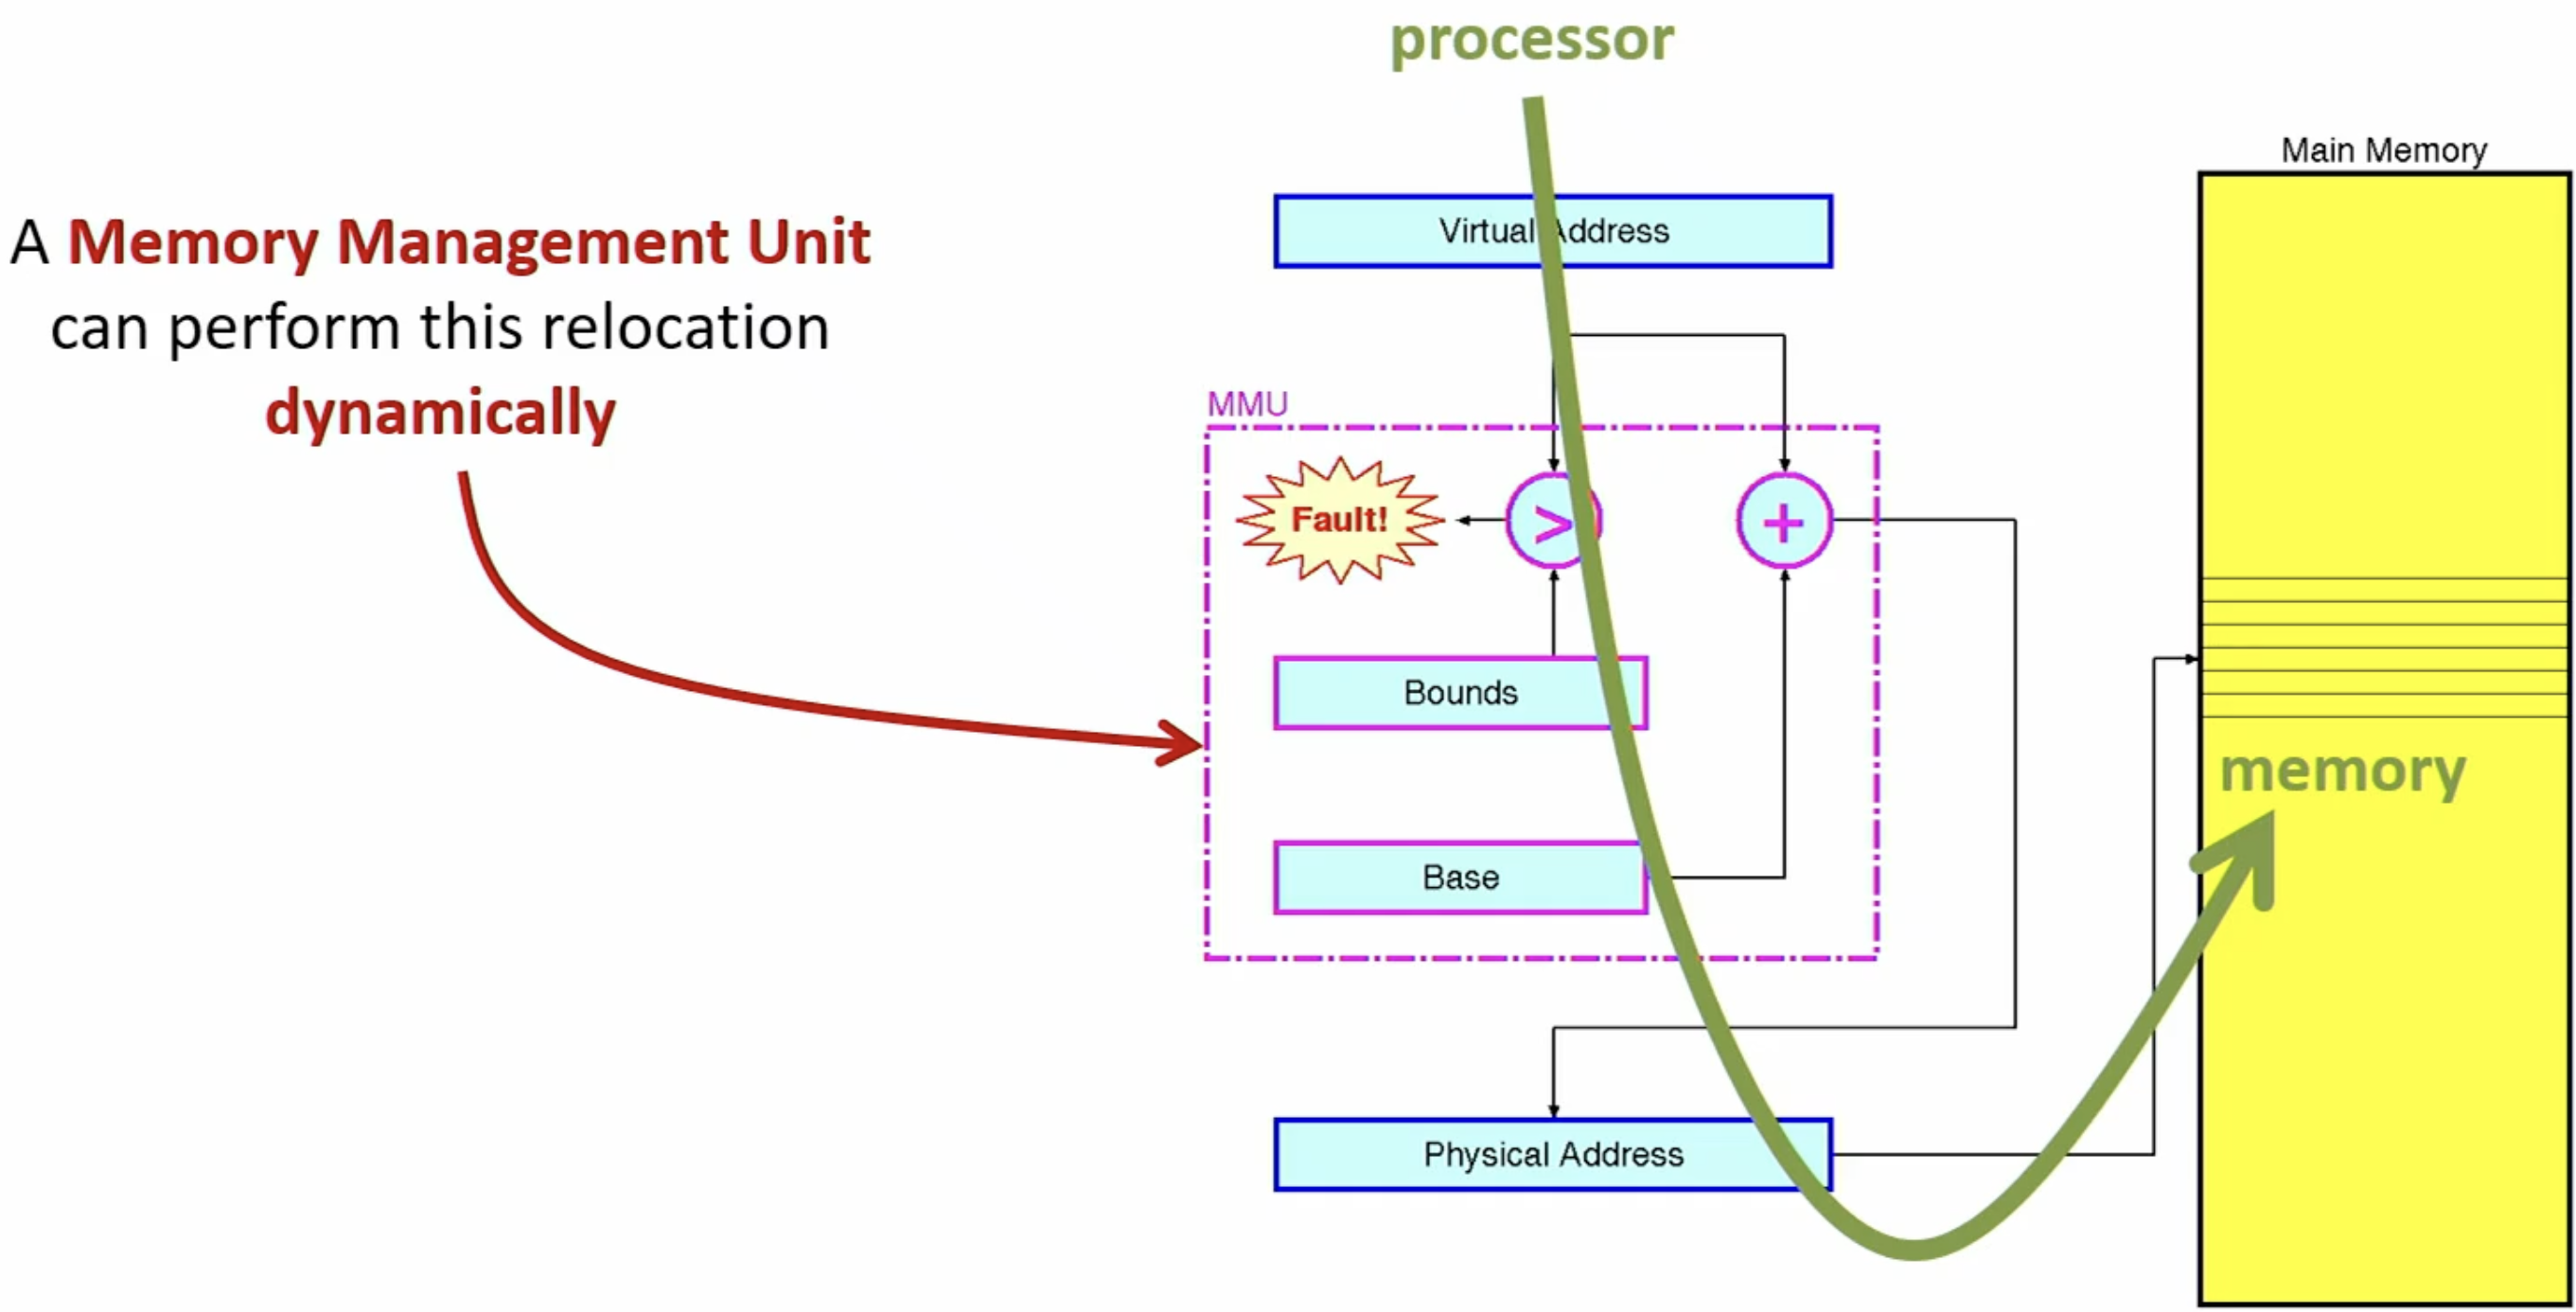
\includegraphics[width=0.65\textwidth]{chapters/chapter3c/images/MMU.png}
\end{center}
\begin{itemize}
    \item[-] \textbf{Base Register:} Holds the starting physical address of the process's memory.
    \item[-] \textbf{Bounds Register:} Defines the limit or size of the memory allocated to the process.
    \item[-] \textbf{Translation Process:}
    \begin{enumerate}
        \item The processor generates a \textit{virtual address}.
        \item The MMU checks if the virtual address exceeds the value in the \textit{Bounds Register}.
        \begin{itemize}
            \item If it exceeds, a \textbf{fault} is raised, preventing illegal memory access.
            \item Otherwise, the MMU adds the \textit{Base Register} value to the virtual address, producing the \textit{physical address}.
        \end{itemize}
        \item The \textit{physical address} is used to access the main memory.
    \end{enumerate}
\end{itemize}

This mechanism ensures process isolation and protects the system against unauthorized memory access, as only addresses within the defined bounds can be accessed. The dynamic nature of this relocation is key to supporting multitasking and efficient memory utilization.
\newpage
\subsection{Memory Management Unit (MMU)}
The \textbf{Memory Management Unit (MMU)} is a critical hardware component that facilitates the translation of \textit{virtual addresses} generated by the processor into \textit{physical addresses} used by the memory. This process is essential for efficient memory management in modern computer systems.

\begin{center}
    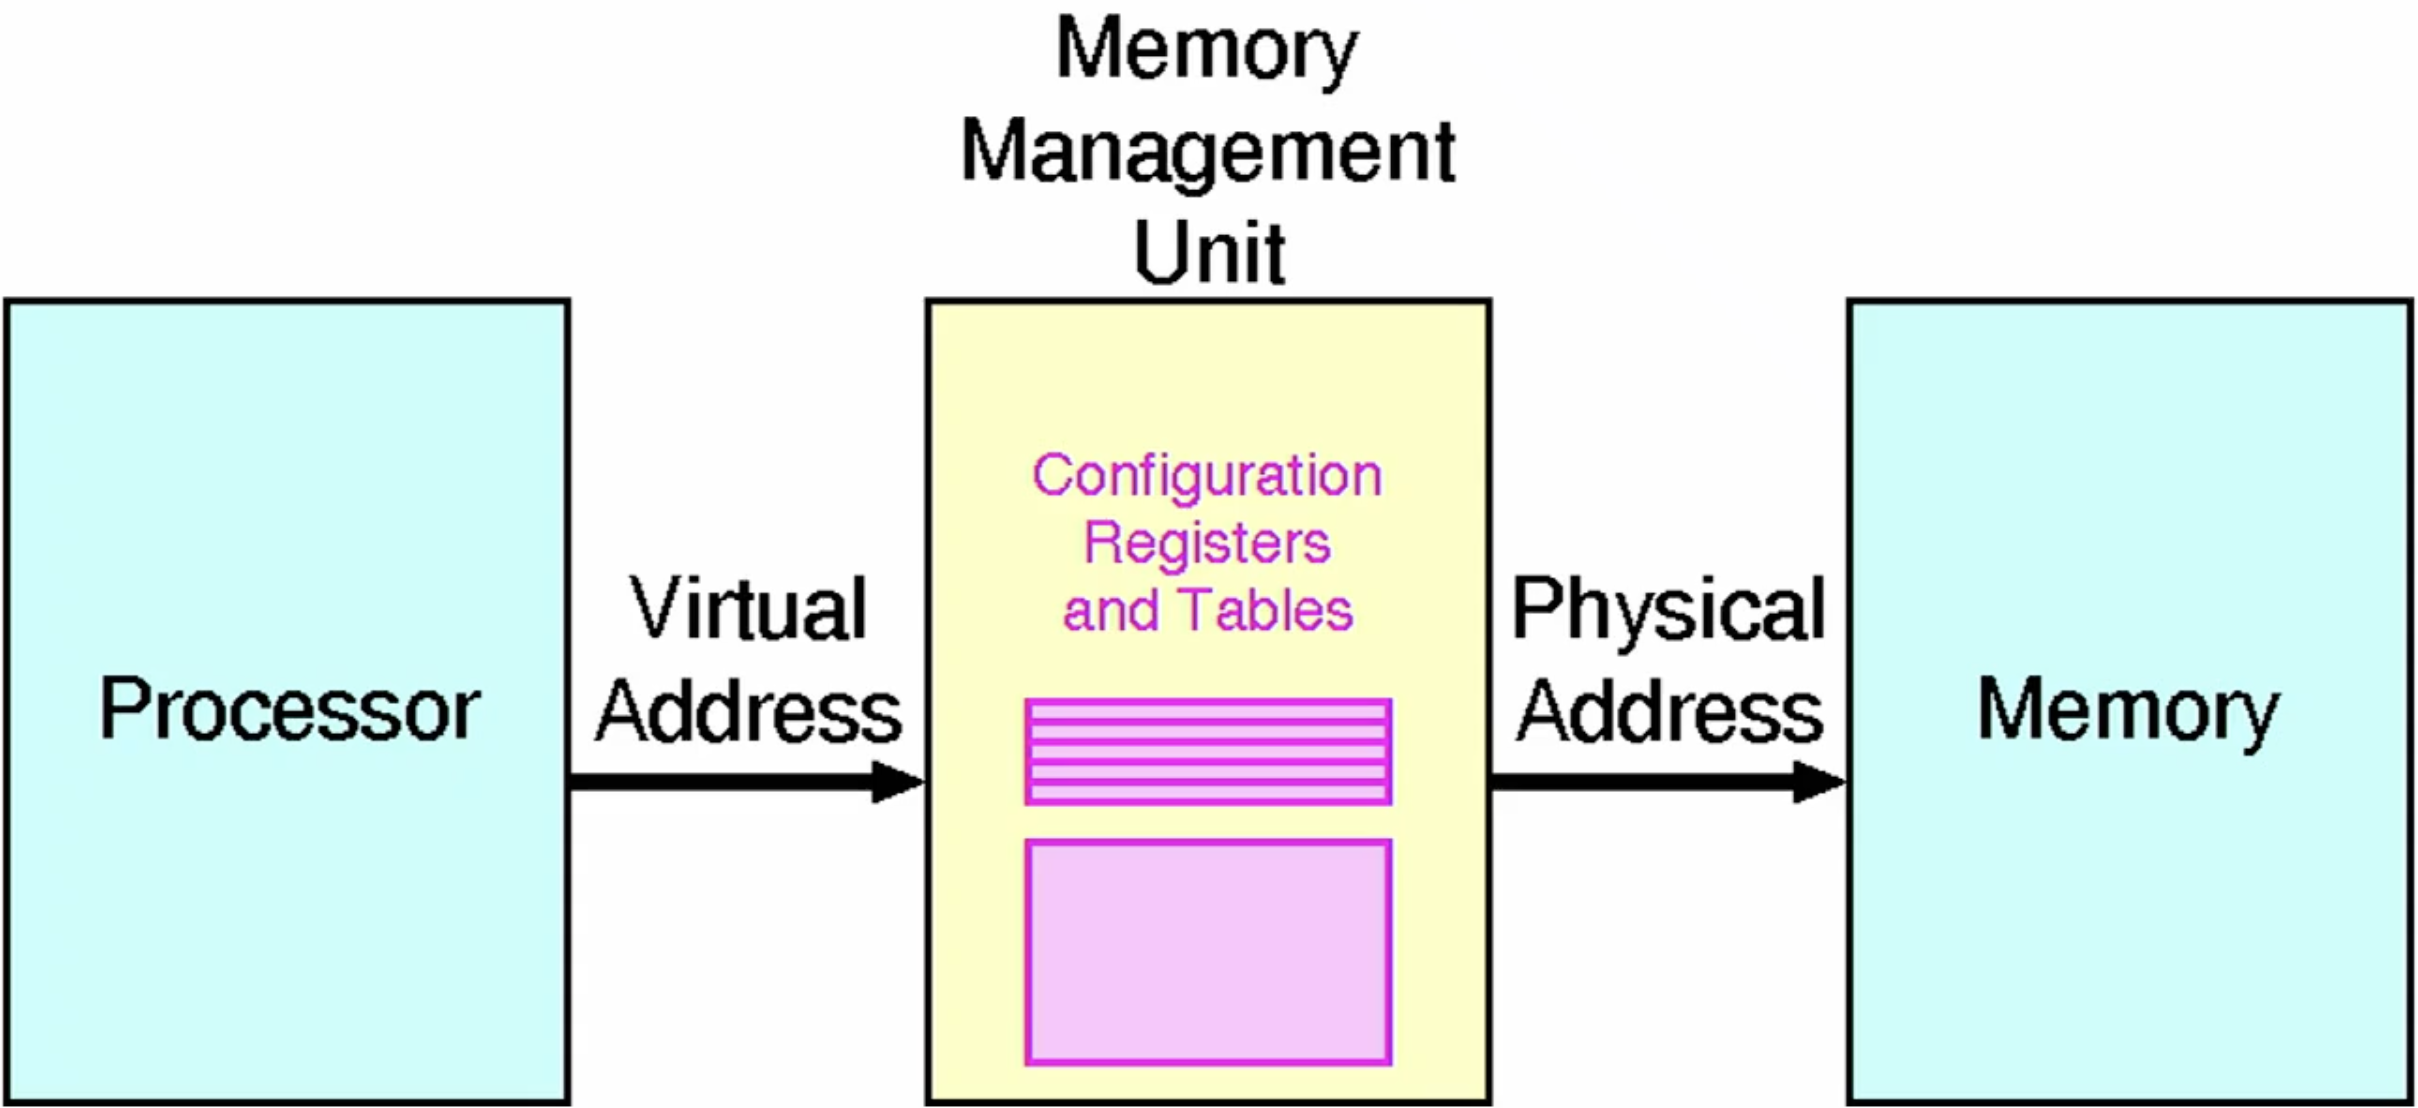
\includegraphics[width=0.65\textwidth]{chapters/chapter3c/images/MMU2.png}
\end{center}
\begin{itemize}
    \item[-] \textbf{Virtual Address:} Generated by the processor, representing a logical view of memory.
    \item[-] \textbf{Physical Address:} The actual address in the main memory where data is stored.
    \item[-] \textbf{Key Components:}
    \begin{enumerate}
        \item \textit{Configuration Registers:} Store information such as base addresses, bounds, and page tables.
        \item \textit{Translation Tables:} Facilitate the mapping of virtual to physical addresses.
    \end{enumerate}
    \item[-] \textbf{Process Overview:}
    \begin{enumerate}
        \item The processor generates a \textit{virtual address}.
        \item The MMU uses its configuration registers and translation tables to map the virtual address to a physical address.
        \item The mapped physical address is used to access data in the main memory.
    \end{enumerate}
\end{itemize}

\subsection{Program Relocation with Virtual Memory}
Virtual memory provides a powerful abstraction that decouples a program's logical memory view from the physical memory of the system. This flexibility is achieved by isolating programs from the underlying physical memory addresses, allowing dynamic relocation of programs without affecting their execution.
\begin{center}
    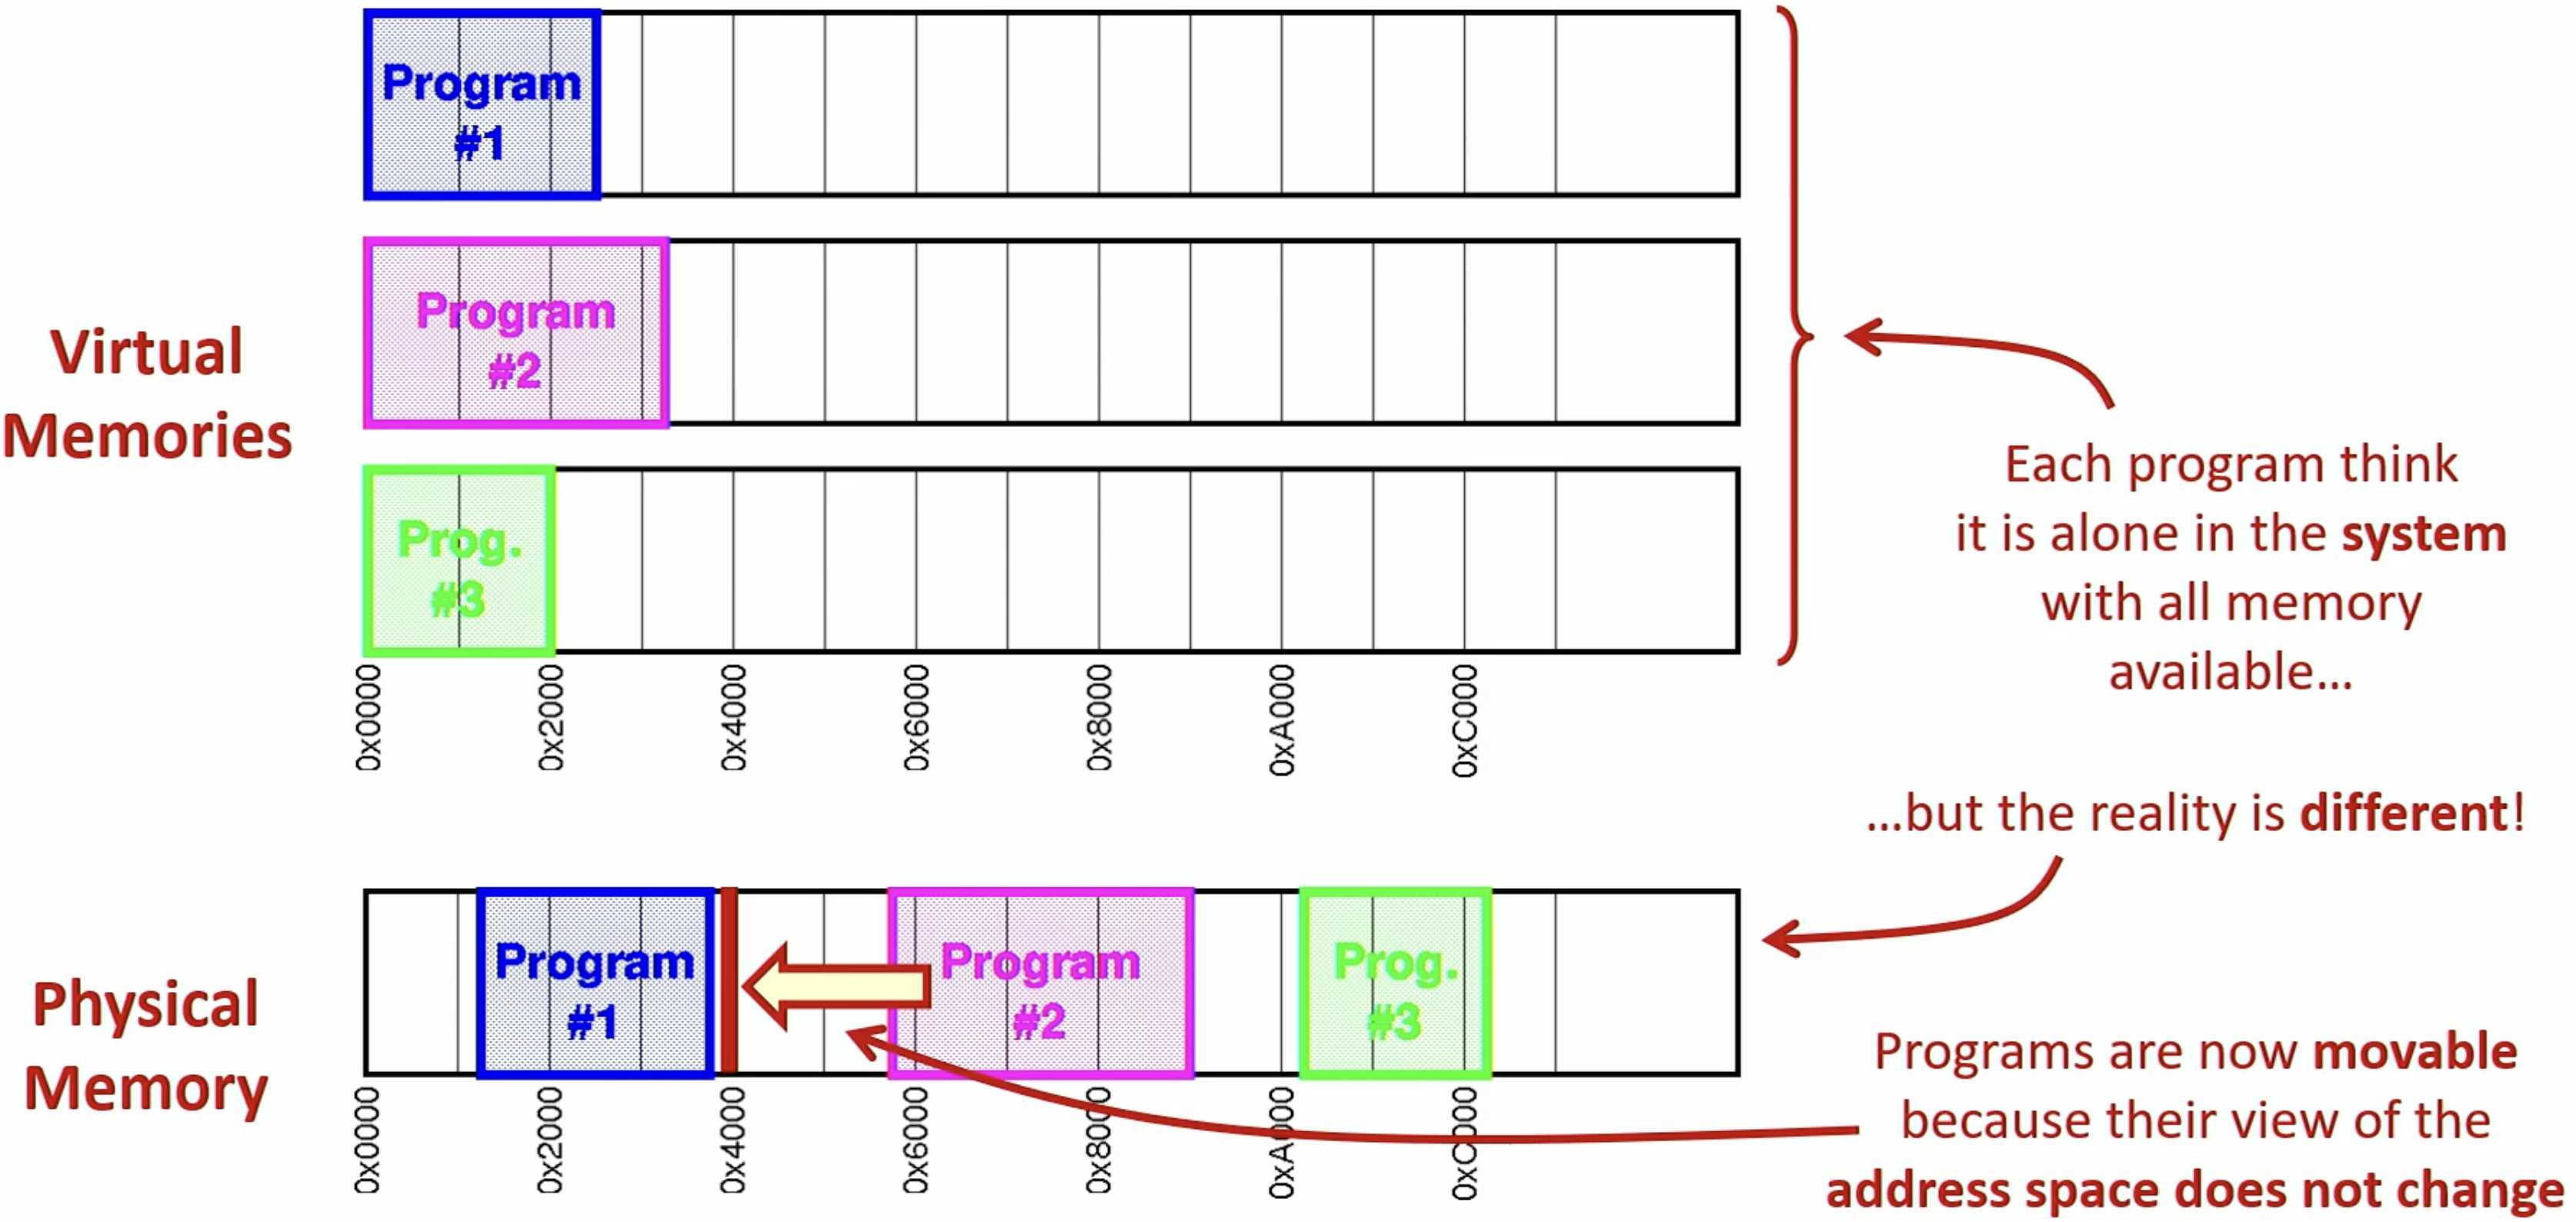
\includegraphics[width=0.65\textwidth]{chapters/chapter3c/images/virtual.png}
\end{center}
\begin{itemize}
    \item \textbf{Independent Address Spaces:} Each program is assigned its own virtual address space, creating the illusion that it has exclusive access to the entire memory. The program is unaware of its actual location in physical memory.
    \item \textbf{Program Relocation:} Since a program only interacts with its virtual address space, the operating system can freely move its physical location in memory as needed. This movement, known as \textit{relocation}, can occur during execution or at load time.
    \item \textbf{Benefits of Relocation:}
    \begin{itemize}
        \item \textit{Efficient Memory Use:} Programs can be compacted to free up contiguous physical memory for other processes.
        \item \textit{Load Balancing:} Active programs can be repositioned to optimize memory access speed or reduce fragmentation.
        \item \textit{Seamless Execution:} Since the memory translation is handled by the hardware (e.g., the Memory Management Unit, MMU), the program remains unaware of any changes in its physical location.
    \end{itemize}
\end{itemize}

\section{Relocation in Hardware: Base and Bounds MMU}
The Base and Bounds MMU (Memory Management Unit) is a hardware mechanism designed to facilitate memory relocation. It operates by performing two key actions on a virtual address provided by a process:
\begin{center}
    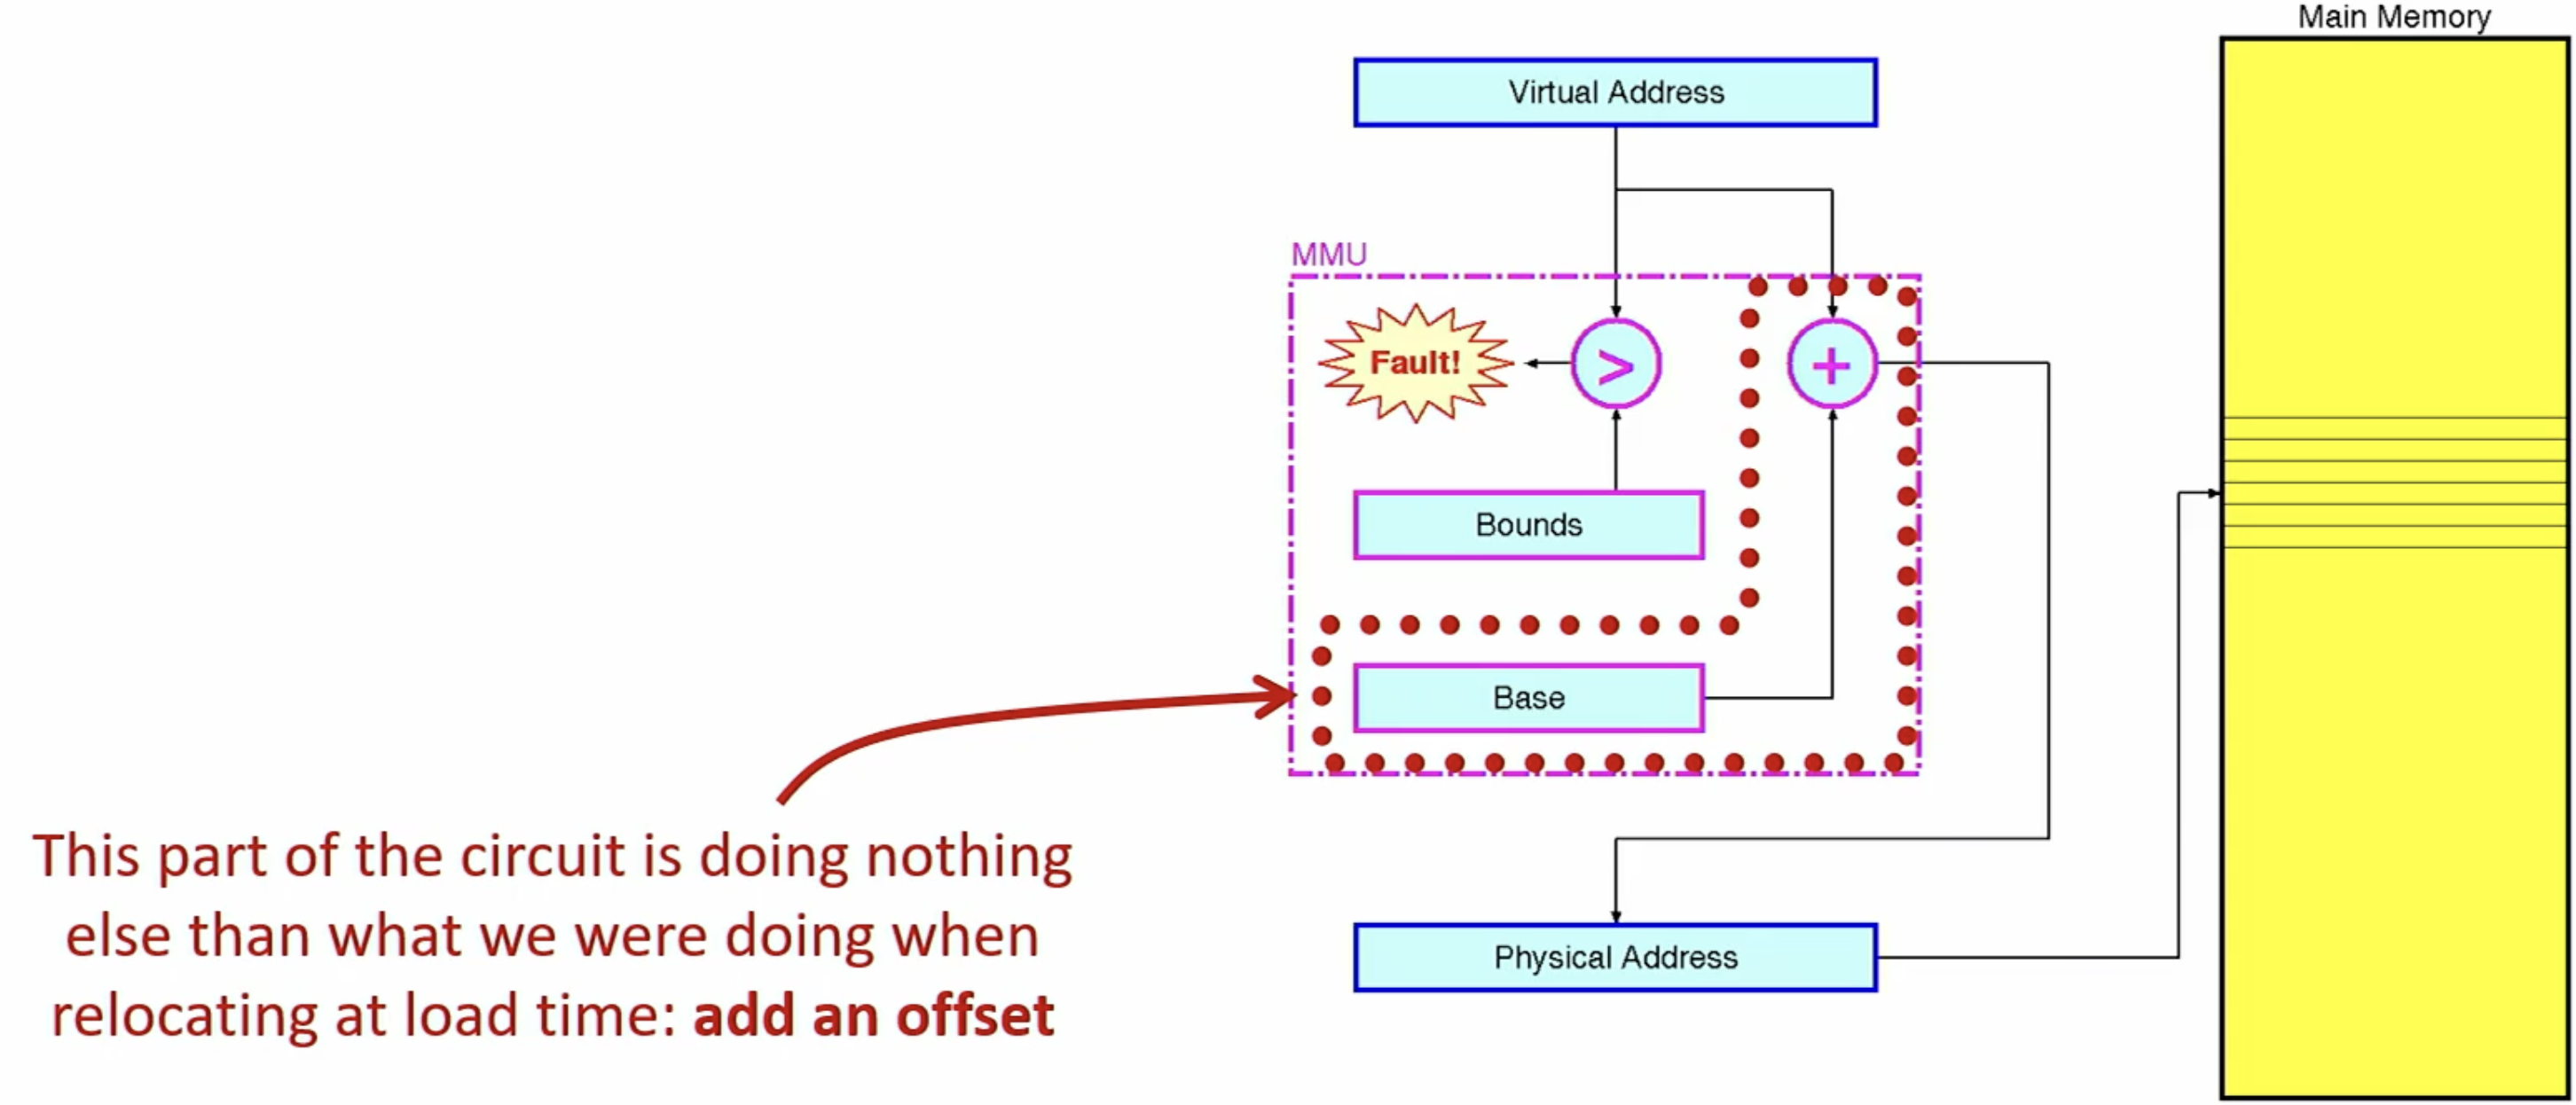
\includegraphics[width=0.65\textwidth]{chapters/chapter3c/images/relocation.png}
\end{center}
\begin{itemize}
    \item \textbf{Bounds Check:} The virtual address is compared with the \texttt{Bounds} register to ensure it is within the allowable range. If the virtual address exceeds the bounds, a fault is triggered, preventing unauthorized access.
    \item \textbf{Offset Addition:} If the virtual address is valid, it is added to the value in the \texttt{Base} register. This offset addition translates the virtual address into a physical address, which is then used to access the main memory.
\end{itemize}

\subsection{Preventing Overreach in Virtual and Physical Memory}
In systems using virtual memory, it is critical to ensure that programs remain within their allocated address spaces. If a program accesses memory beyond its assigned virtual boundaries, it risks overlapping with another program's memory. This can lead to severe security and stability issues.
\begin{center}
    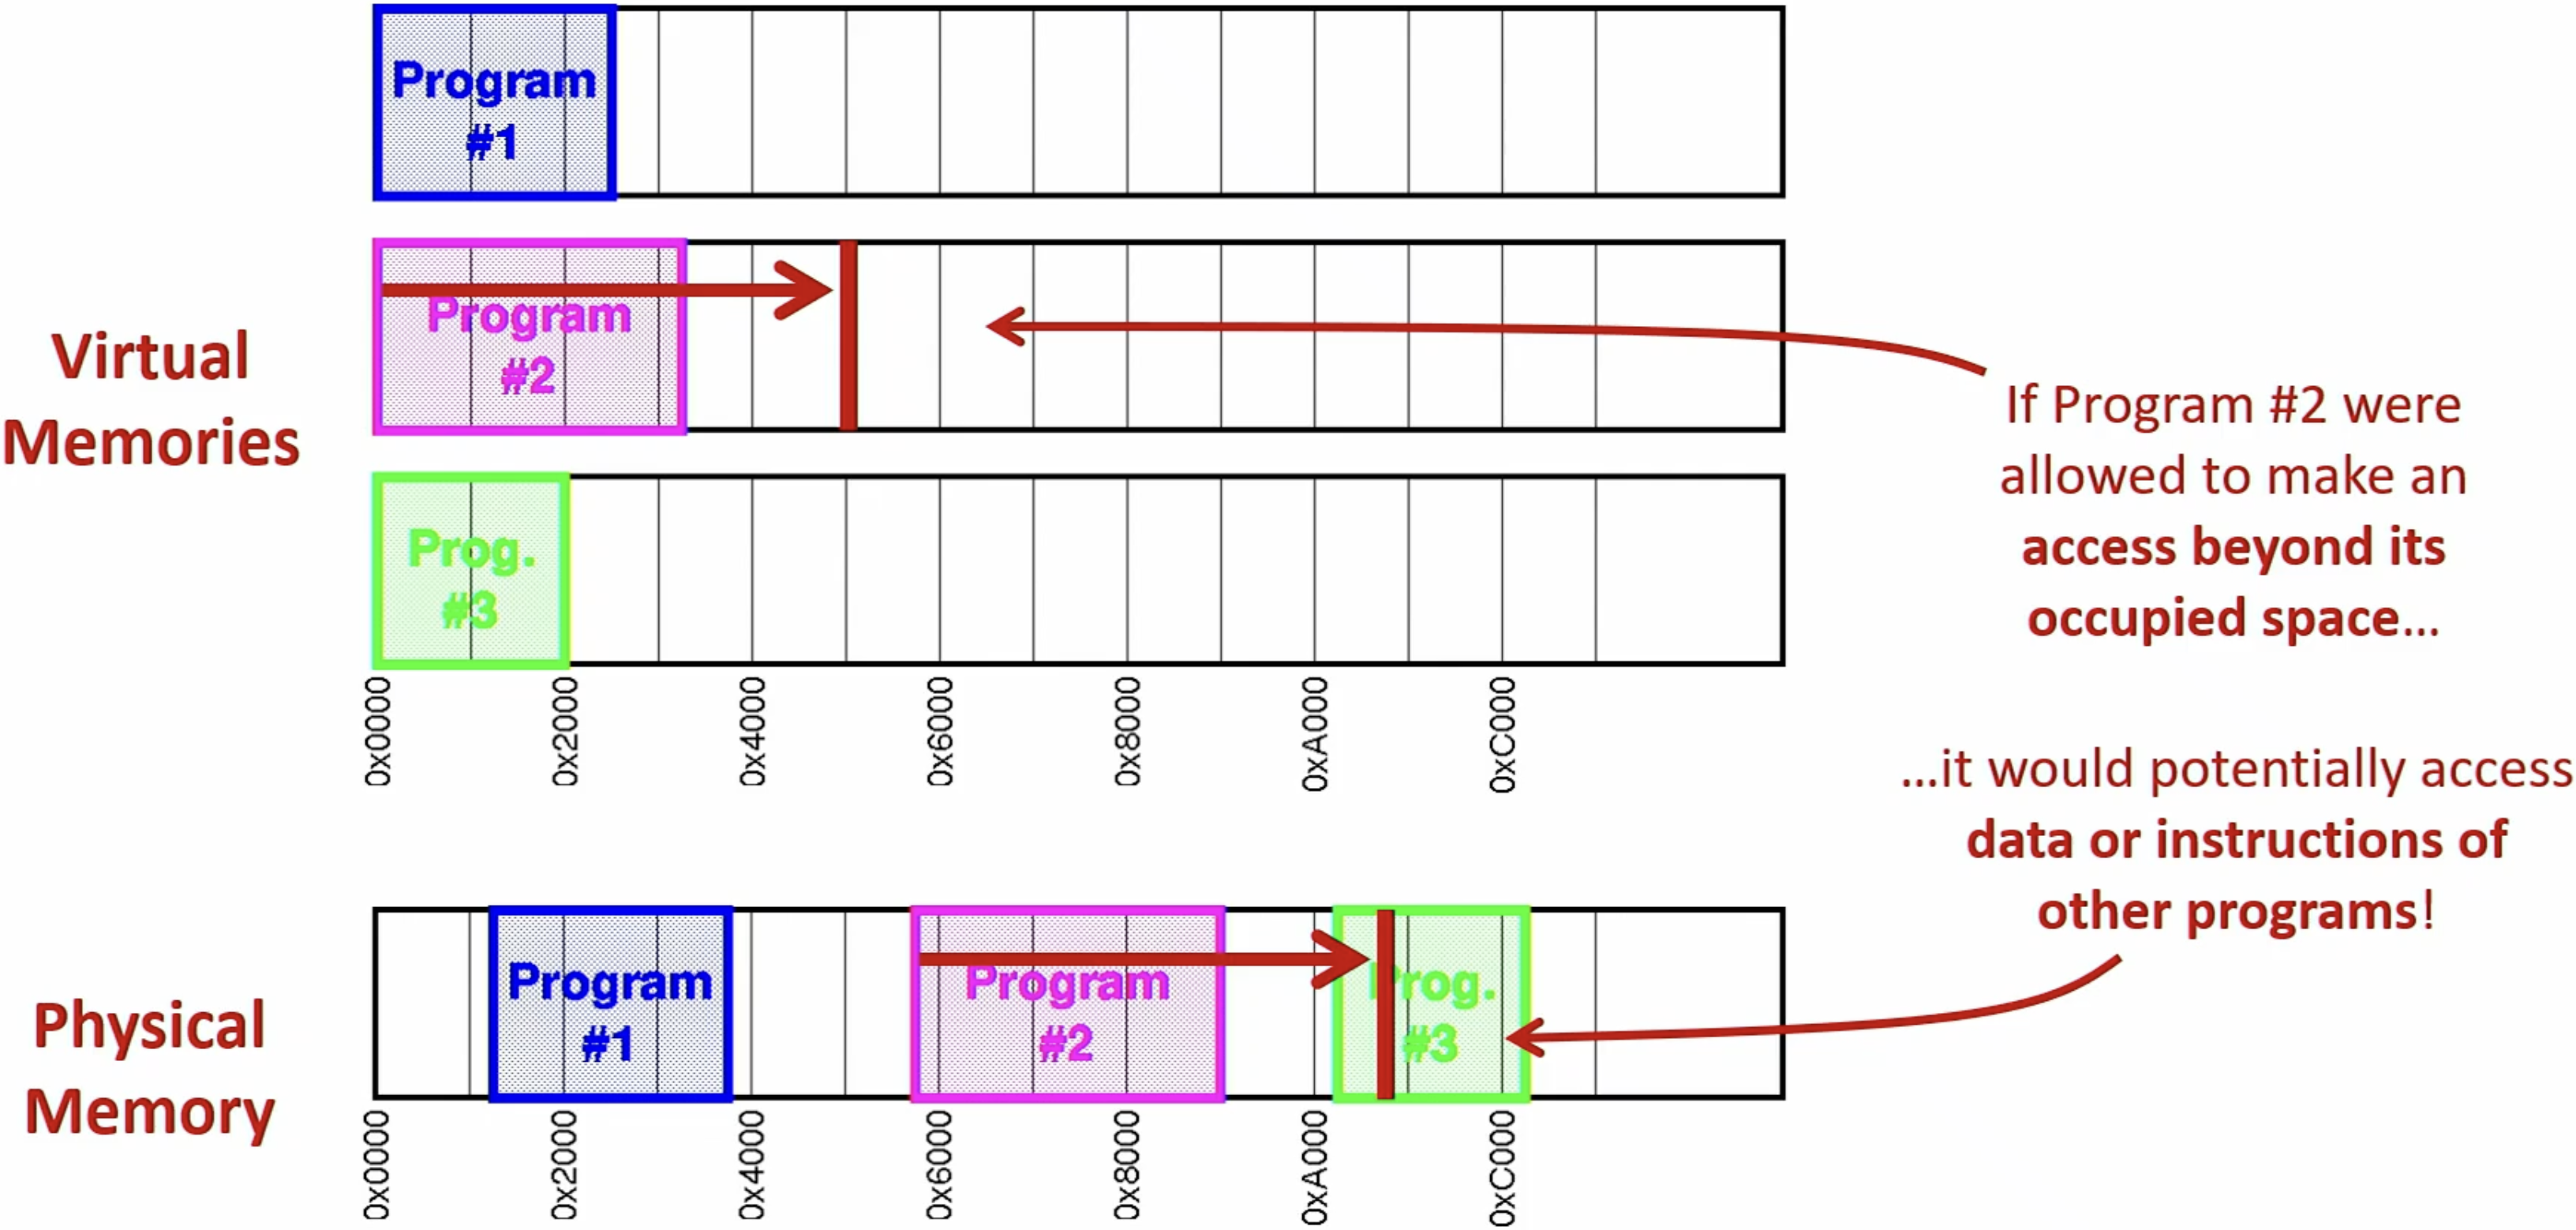
\includegraphics[width=0.65\textwidth]{chapters/chapter3c/images/fault.png}
\end{center}
\begin{itemize}
    \item[-] \textbf{Virtual Memory Overreach:} Each program is given its own virtual address space. However, if a program attempts to access an address outside its bounds, it could inadvertently access data or instructions from another program. This can compromise the integrity of both programs.
    \item[-] \textbf{MMU Checks:} To prevent such overreach, the Memory Management Unit (MMU) enforces strict bounds checking. It ensures that all memory accesses fall within the allowed range defined by the program's base and bounds registers. If a memory access is outside these bounds, the MMU generates a fault, preventing the access.
    \item[-] \textbf{Physical Memory Isolation:} Even though programs use virtual addresses, these are translated to physical addresses by the MMU. Proper isolation ensures that physical memory regions assigned to different programs do not overlap, maintaining system stability.
\end{itemize}

This mechanism of bounds checking and fault generation safeguards against unintended interactions between programs and ensures that no program can overwrite or access another program's data.

\subsection{Base and Bounds MMU}

\begin{center} 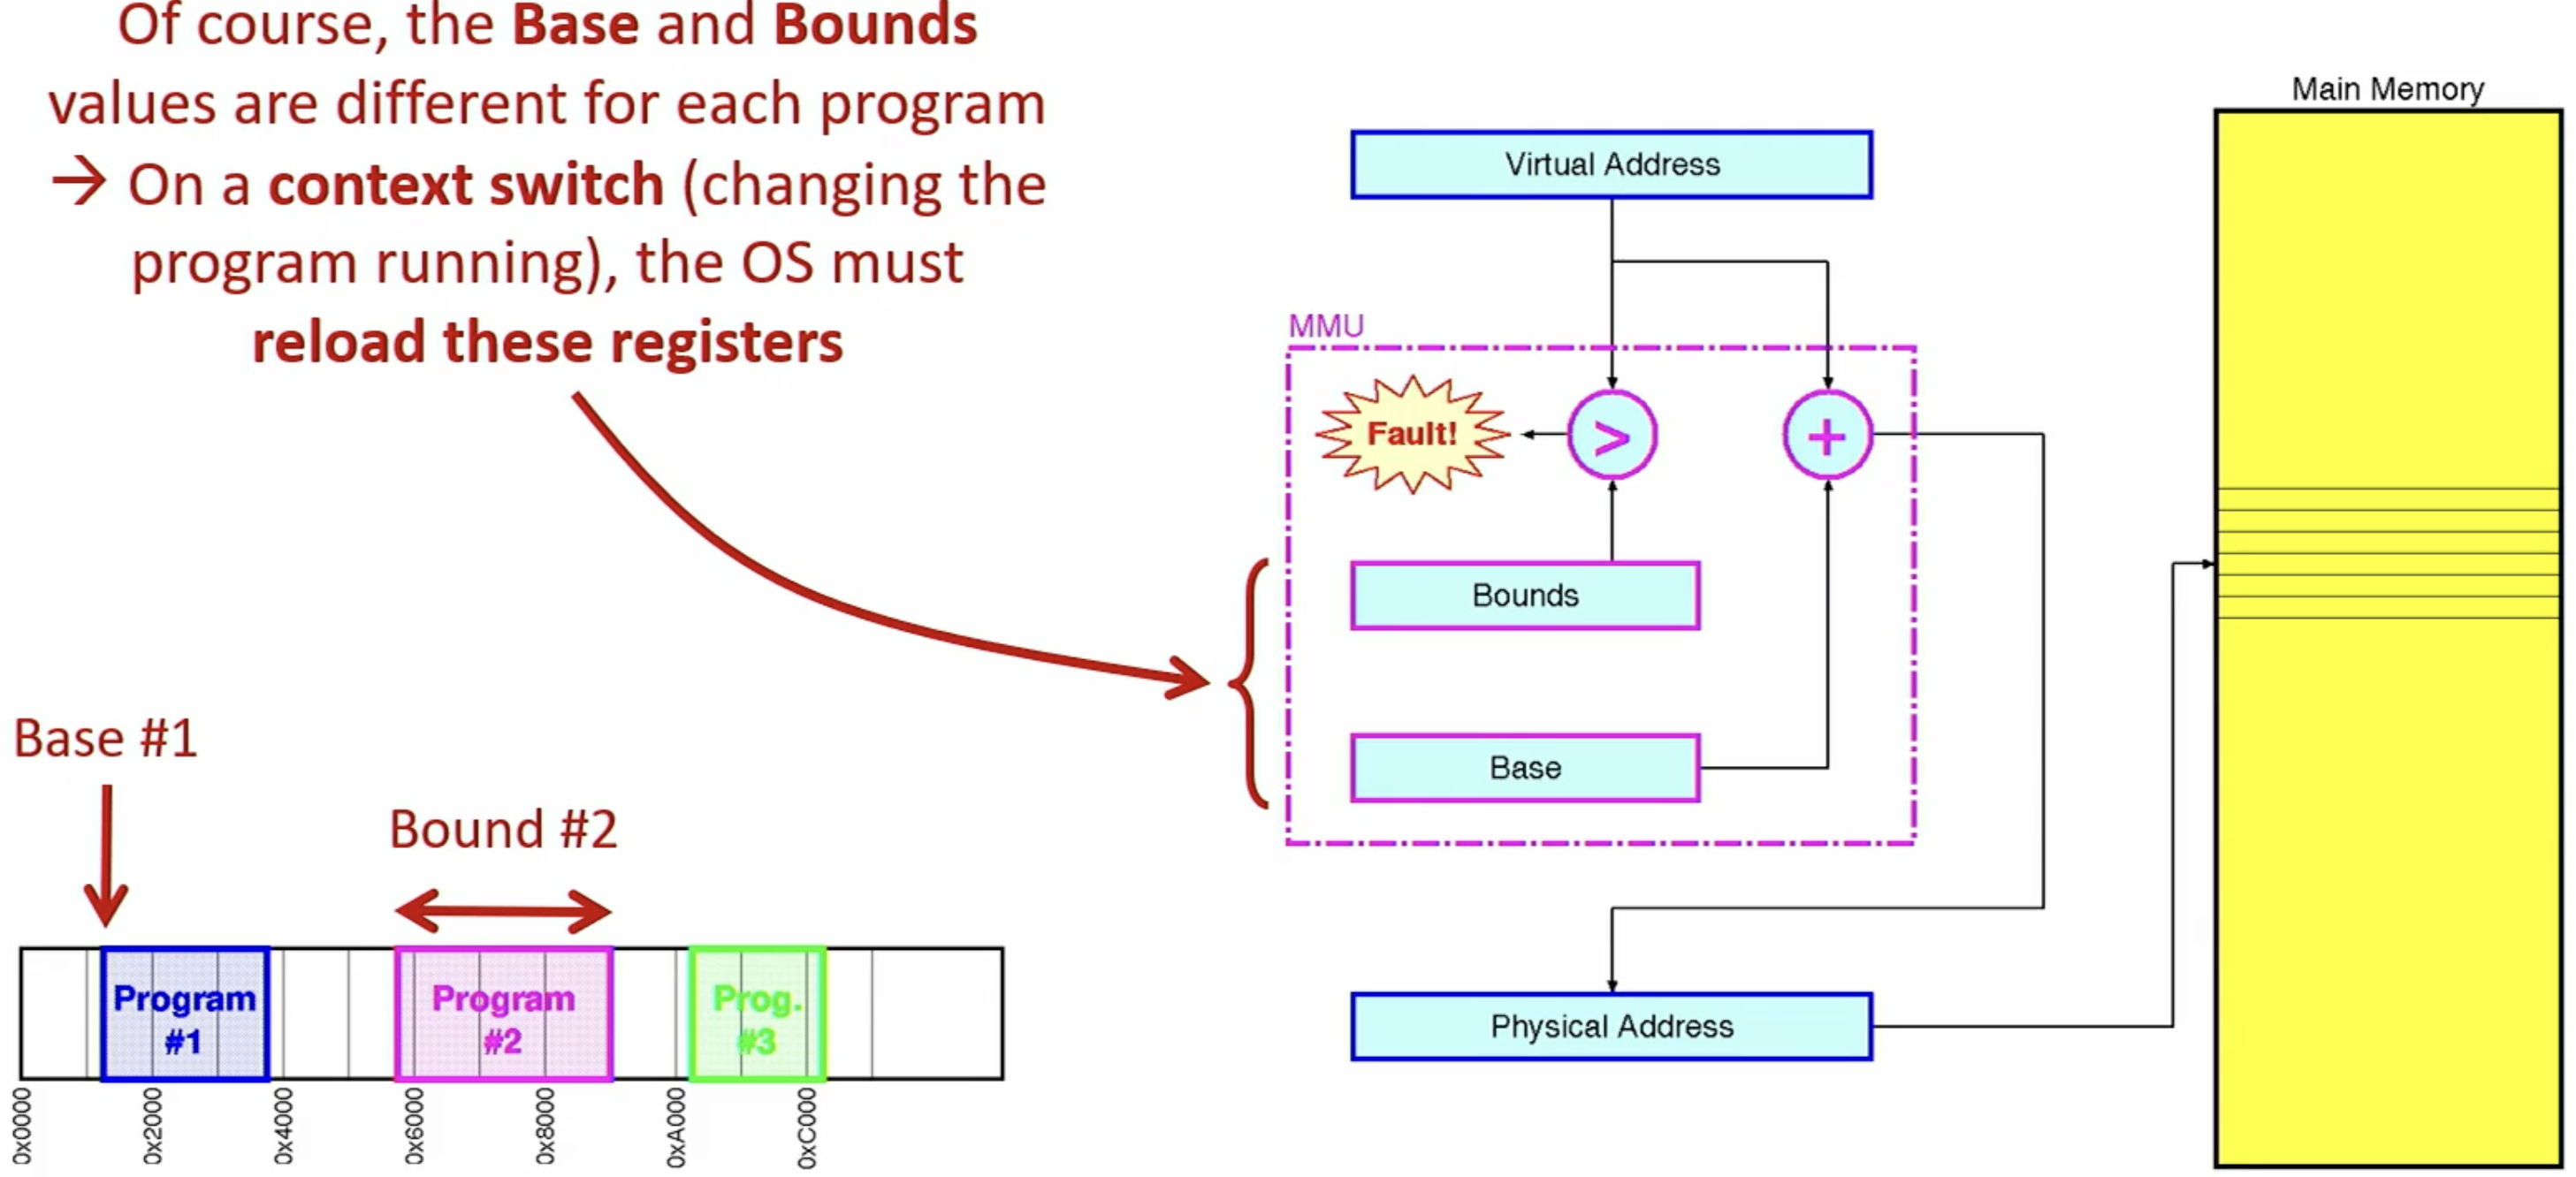
\includegraphics[width=0.65\textwidth]{chapters/chapter3c/images/bb.png} \end{center}

The Base and Bounds mechanism in the MMU defines the memory allocation for a process as follows:

\begin{itemize} \item Base: The starting address of the process's allocated memory. \item Bounds: The upper limit or size of the memory allocated to the process. \end{itemize}

\section{Needs of a Multiprogrammed System}

Multiprogrammed systems require efficient handling of memory and process management to ensure reliability and performance. The key requirements are as follows:

\begin{itemize}
    \item[-] \textbf{Relocation:} Programs must be written without prior knowledge of their location in memory. This ensures flexibility when allocating memory during execution.

    \item[-] \textbf{Protection:} Programs are restricted to access only their own data, safeguarding against interference from other programs. However, this protection mechanism can sometimes be crude, as it often limits each program to a single chunk of memory.

    \item[-] \textbf{Space Management:} When several programs run simultaneously, memory shortages may arise. Effective space allocation strategies are needed, which may involve techniques such as garbage collection and moving programs or data to optimize memory usage.
\end{itemize}

\section{Segmentation and Paging}
\begin{center}
    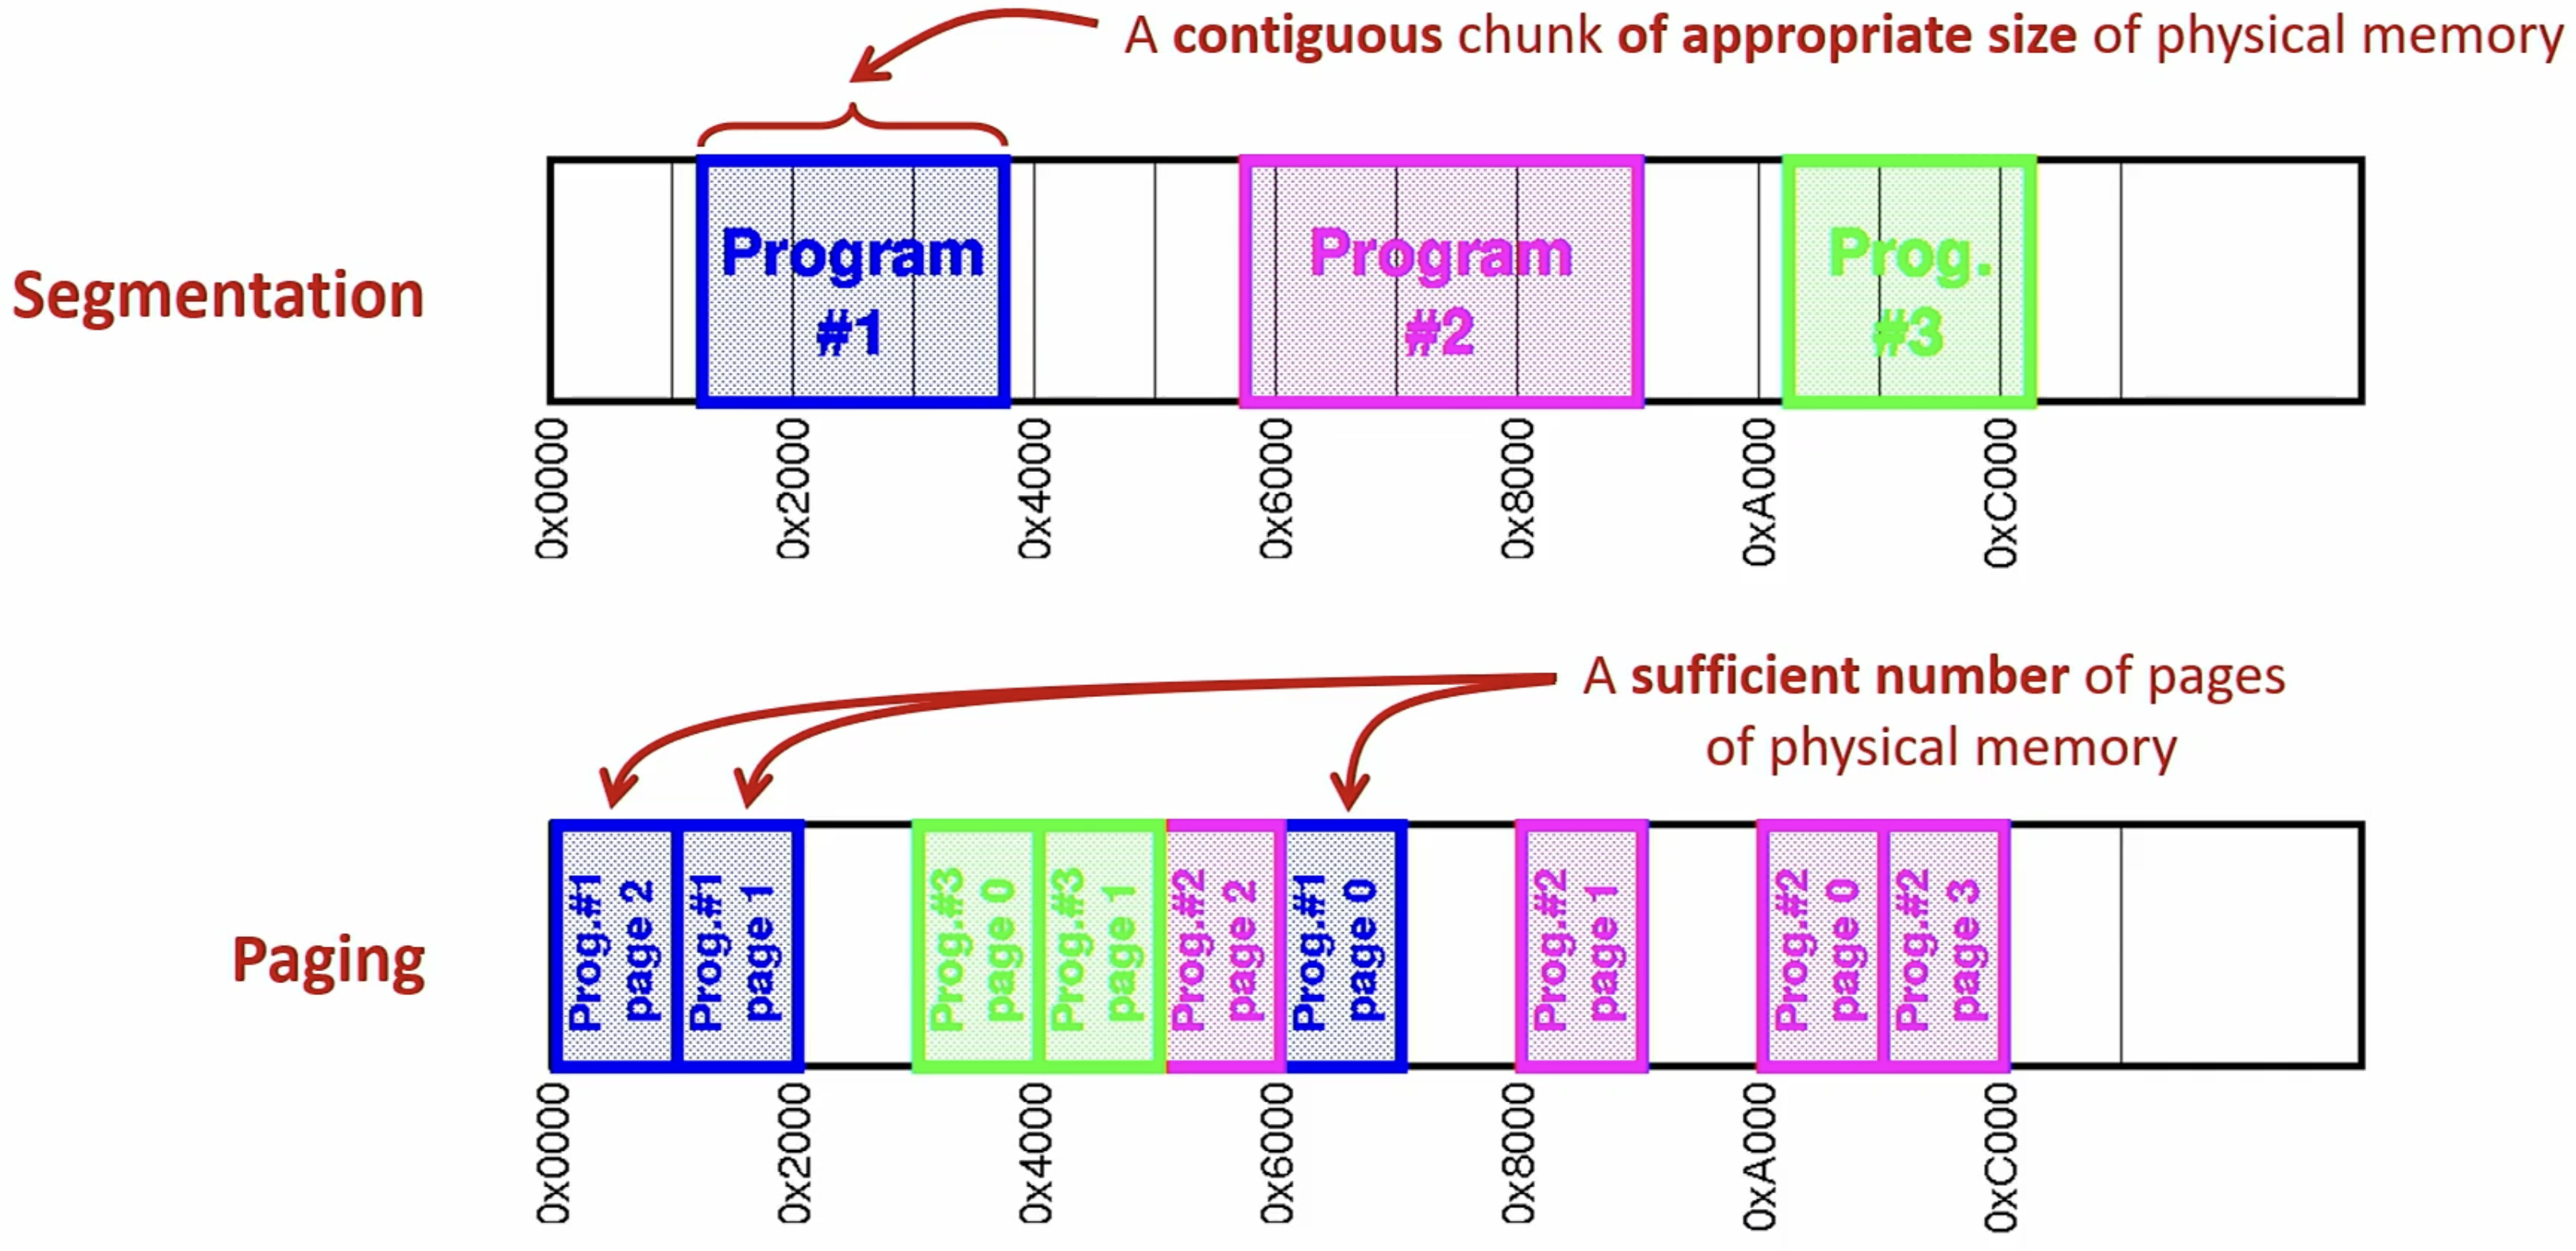
\includegraphics[width=0.65\textwidth]{chapters/chapter3c/images/segPage.png}
\end{center}
\paragraph{Segmentation:} Segmentation, an extension of the Base and Bounds technique, allows memory to be split exactly as needed by each program. Key characteristics include:
\begin{itemize}
    \item[-] Arbitrary starting point of a memory block.
    \item[-] Arbitrary length of memory blocks.
    \item[-] Multiple blocks can be allocated per application.
\end{itemize}

\paragraph{Paging:} Paging divides memory into equal-sized small blocks (e.g., 4–64~KiB) and assigns as many blocks as required to each program. This ensures uniformity in memory allocation.

\subsection{How do we Translate Now?}
Now we need to translate virtual addresses to physical addresses (with our new paging constraints). This process involves the following steps:
\begin{center}
    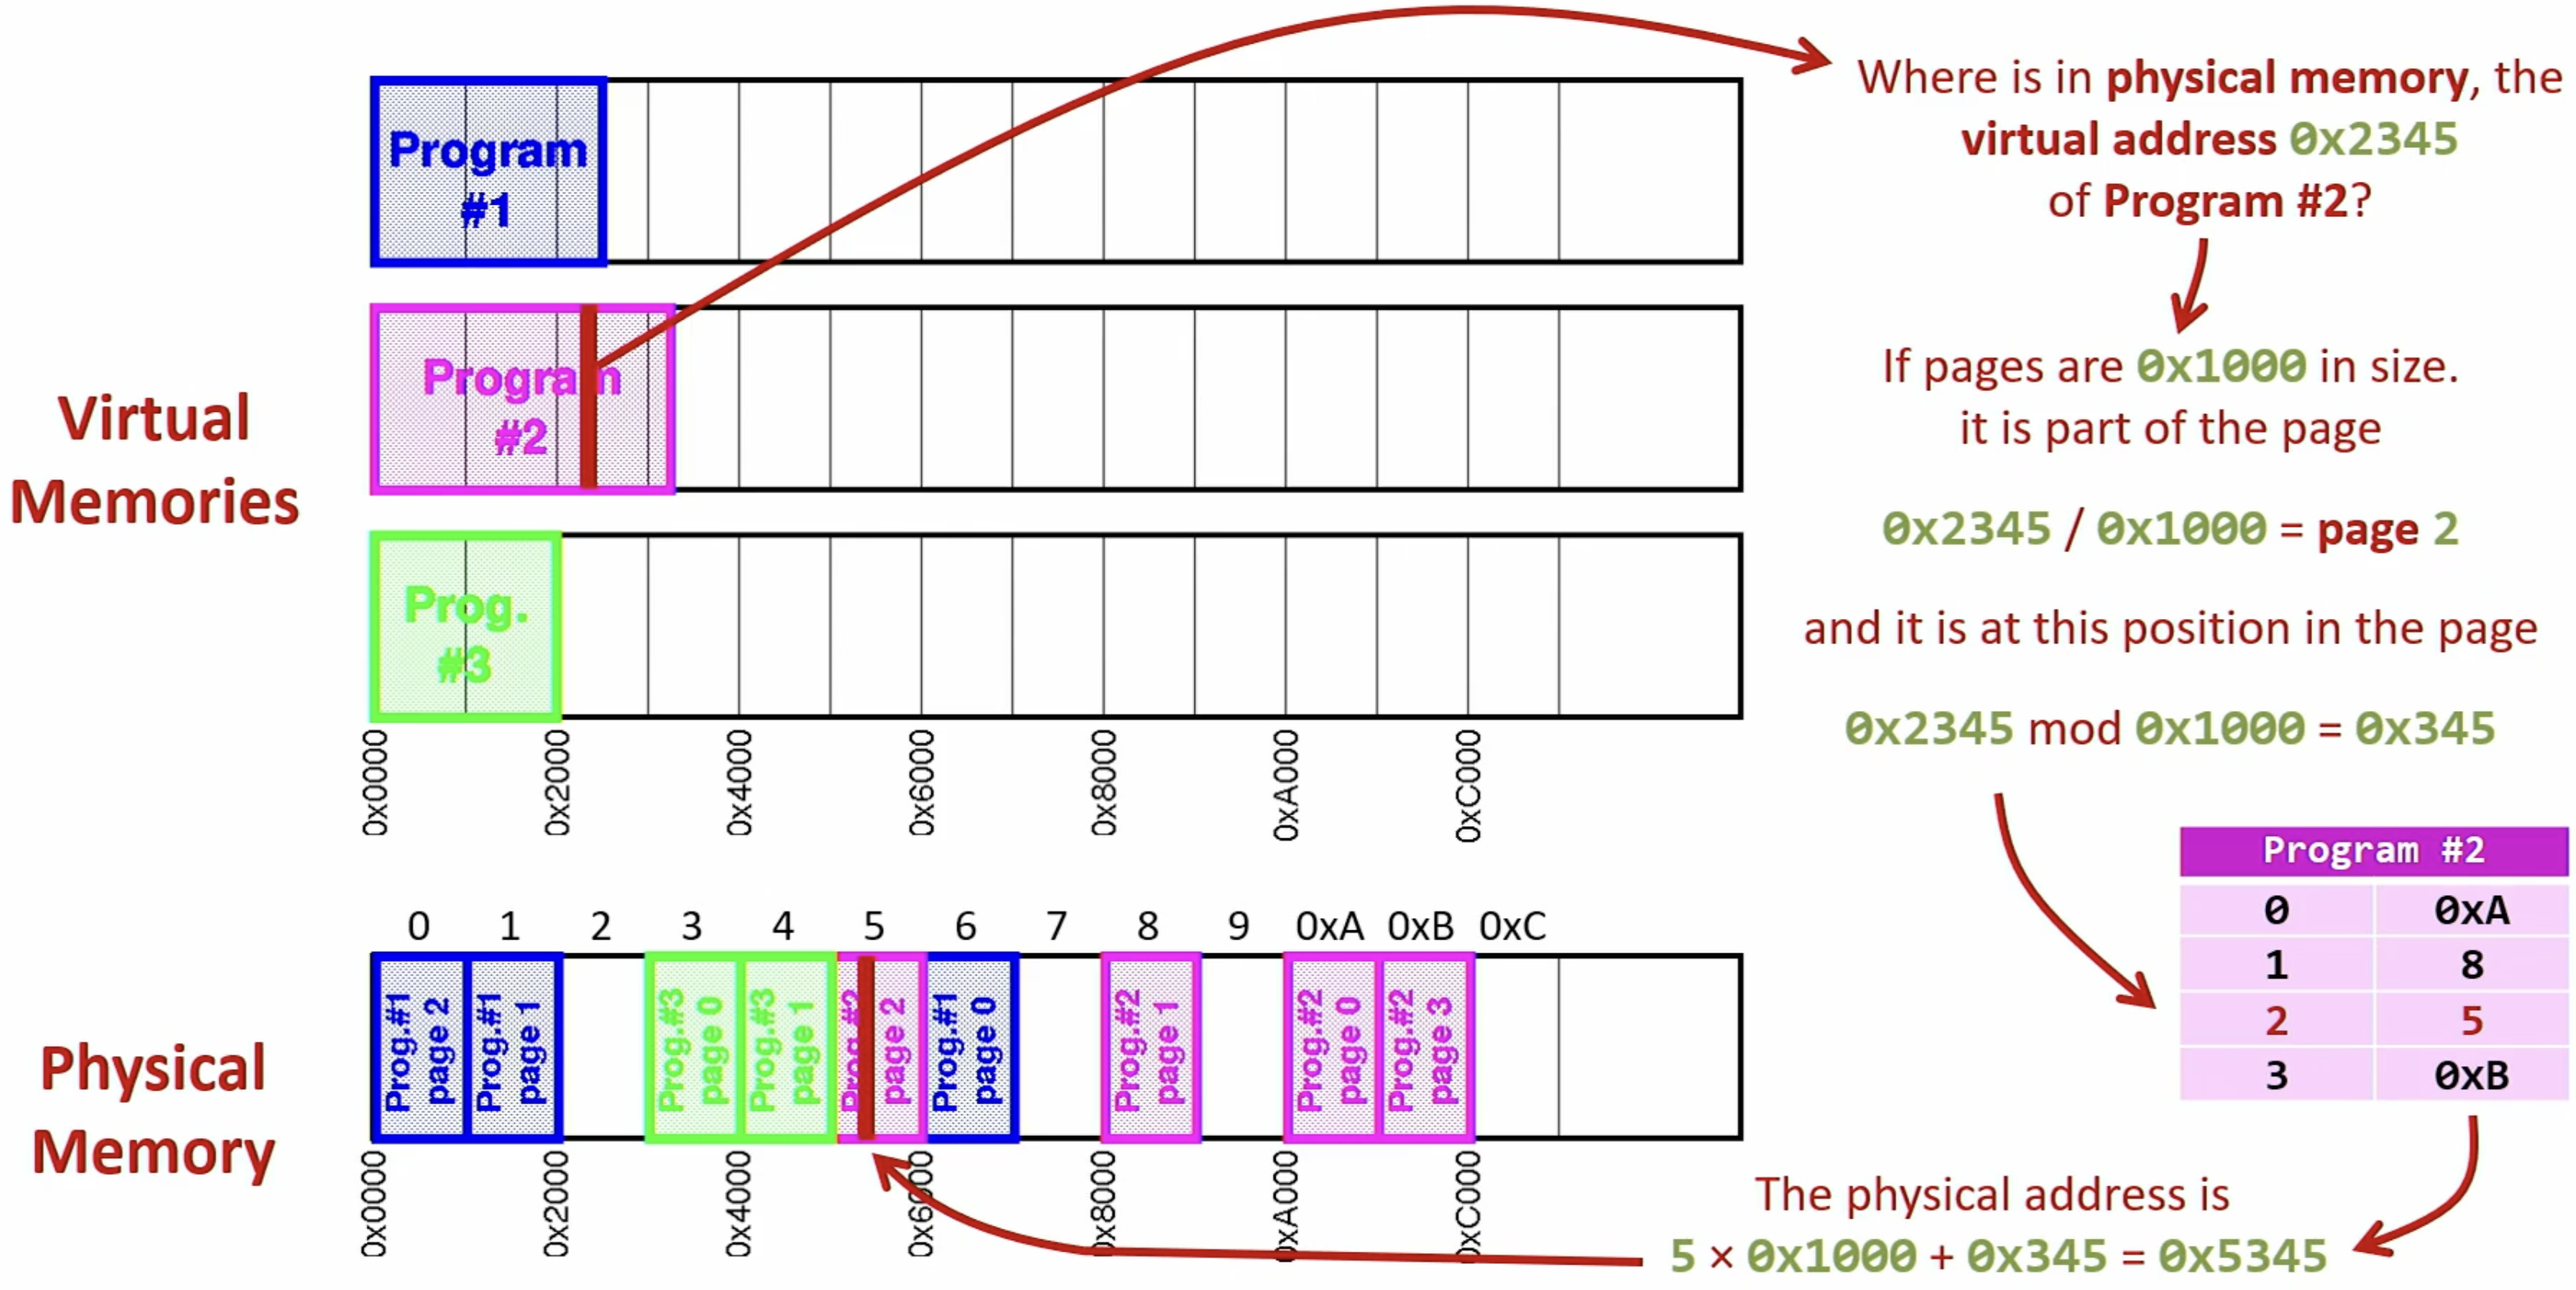
\includegraphics[width=0.65\textwidth]{chapters/chapter3c/images/translate.png}
\end{center}

For example,if the system needs to determine the physical memory location corresponding to the virtual address \texttt{0x2345} of \textbf{Program \#2}. The translation process follows these steps:

\begin{enumerate}
    \item Identify the \textbf{page number} and \textbf{offset} within the virtual address. Assuming page size is known, \texttt{0x2345} translates to a specific page and offset.
    \item Consult the \textbf{page table} for \textbf{Program \#2}, which maps virtual pages to physical pages. For instance:
    \[
    \text{\texttt{Program \#2 Page 0}} \rightarrow \text{\texttt{Physical Page 8}}, \quad
    \text{\texttt{Page 1}} \rightarrow \text{\texttt{Physical Page 9}}
    \]
    \item Use the mapping to locate the physical address. In this example, the virtual address resides in \texttt{Page 0}, which maps to \texttt{Physical Page 8}. Combining the physical page base address with the offset yields the final physical memory address.
\end{enumerate}

Sumarized, to find the physical address, we need to extract the virtual page number and the page offset from the virtual address. The virtual page number is used to look up the corresponding physical frame number in the page table. Finally, the physical address is computed using the formula:
\begin{center}
    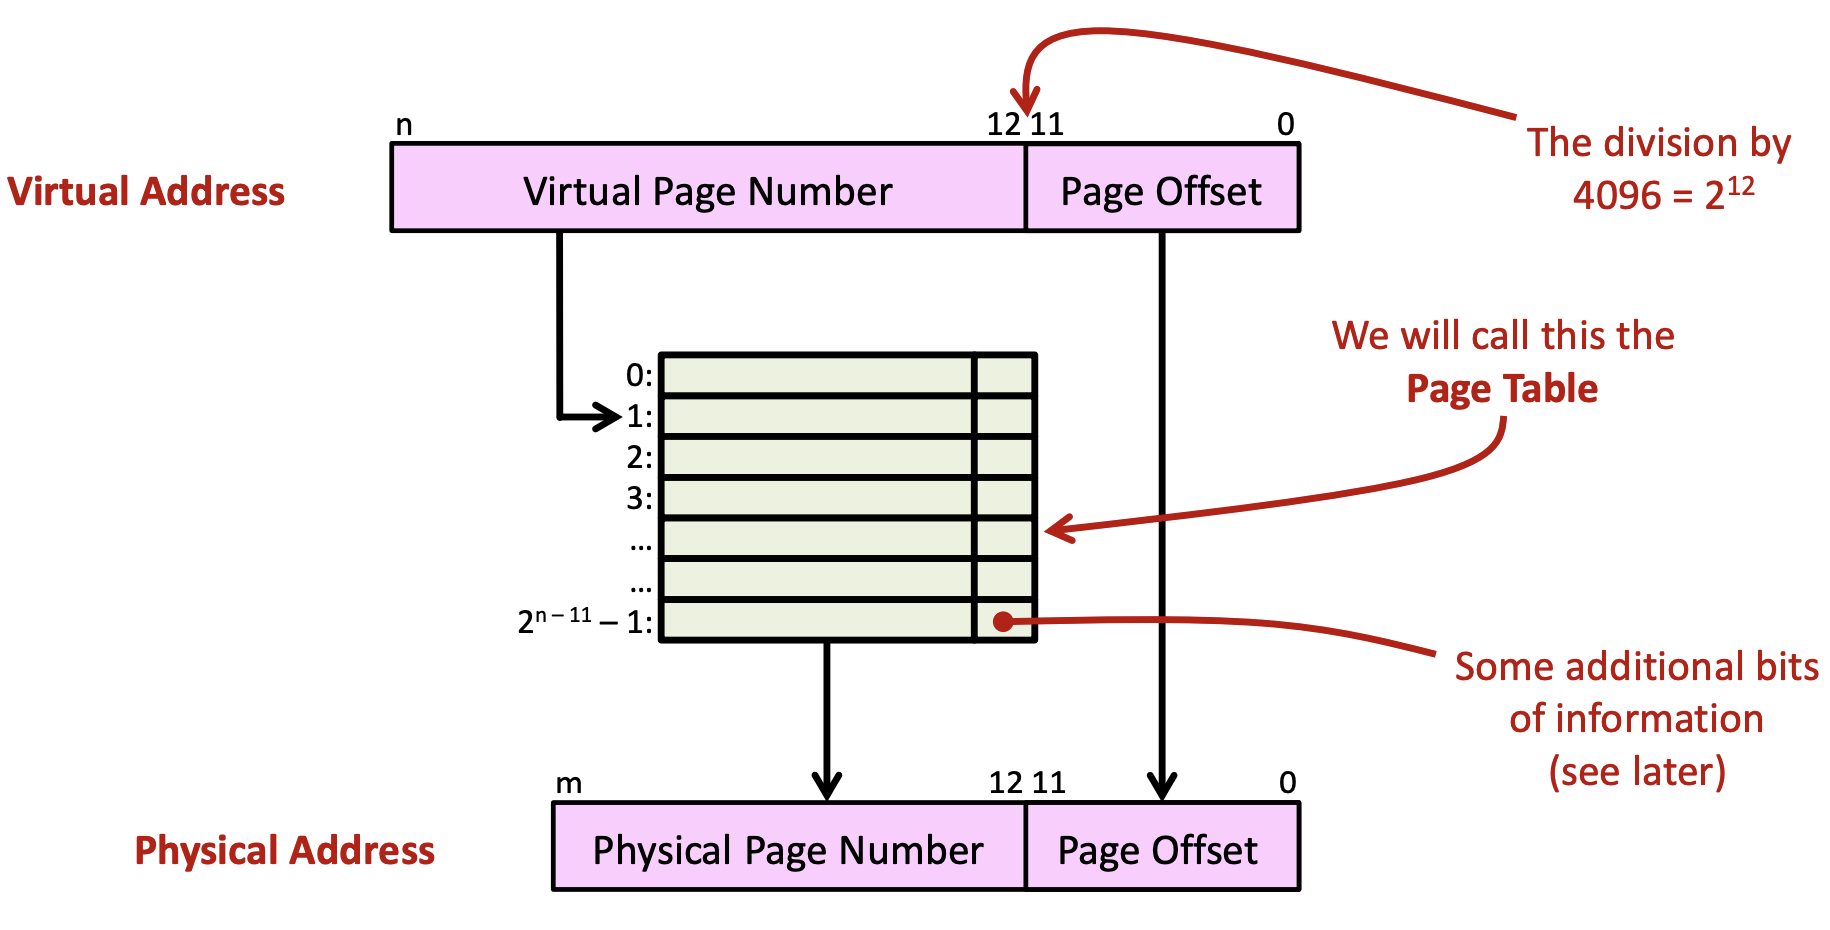
\includegraphics[width=0.65\textwidth]{chapters/chapter3c/images/translate2.png}
\end{center}
\[
\text{Physical Address} = (\text{Physical Frame Number} \times \text{Page Size}) + \text{Page Offset}
\]

where the page offset is directly derived from the virtual address, and the physical frame number is obtained from the page table. The page size is often a power of 2 (for example, \(4 \, \text{KB} = 2^{12}\)), which makes extracting the page offset straightforward as it corresponds to the lower-order bits of the virtual address.
\newpage
\subsection{Virtual Adress Translation in a Paged MMU}
In a paged MMU, the virtual address generated by the processor is translated into a physical address using the page table stored in memory.
\begin{center}
    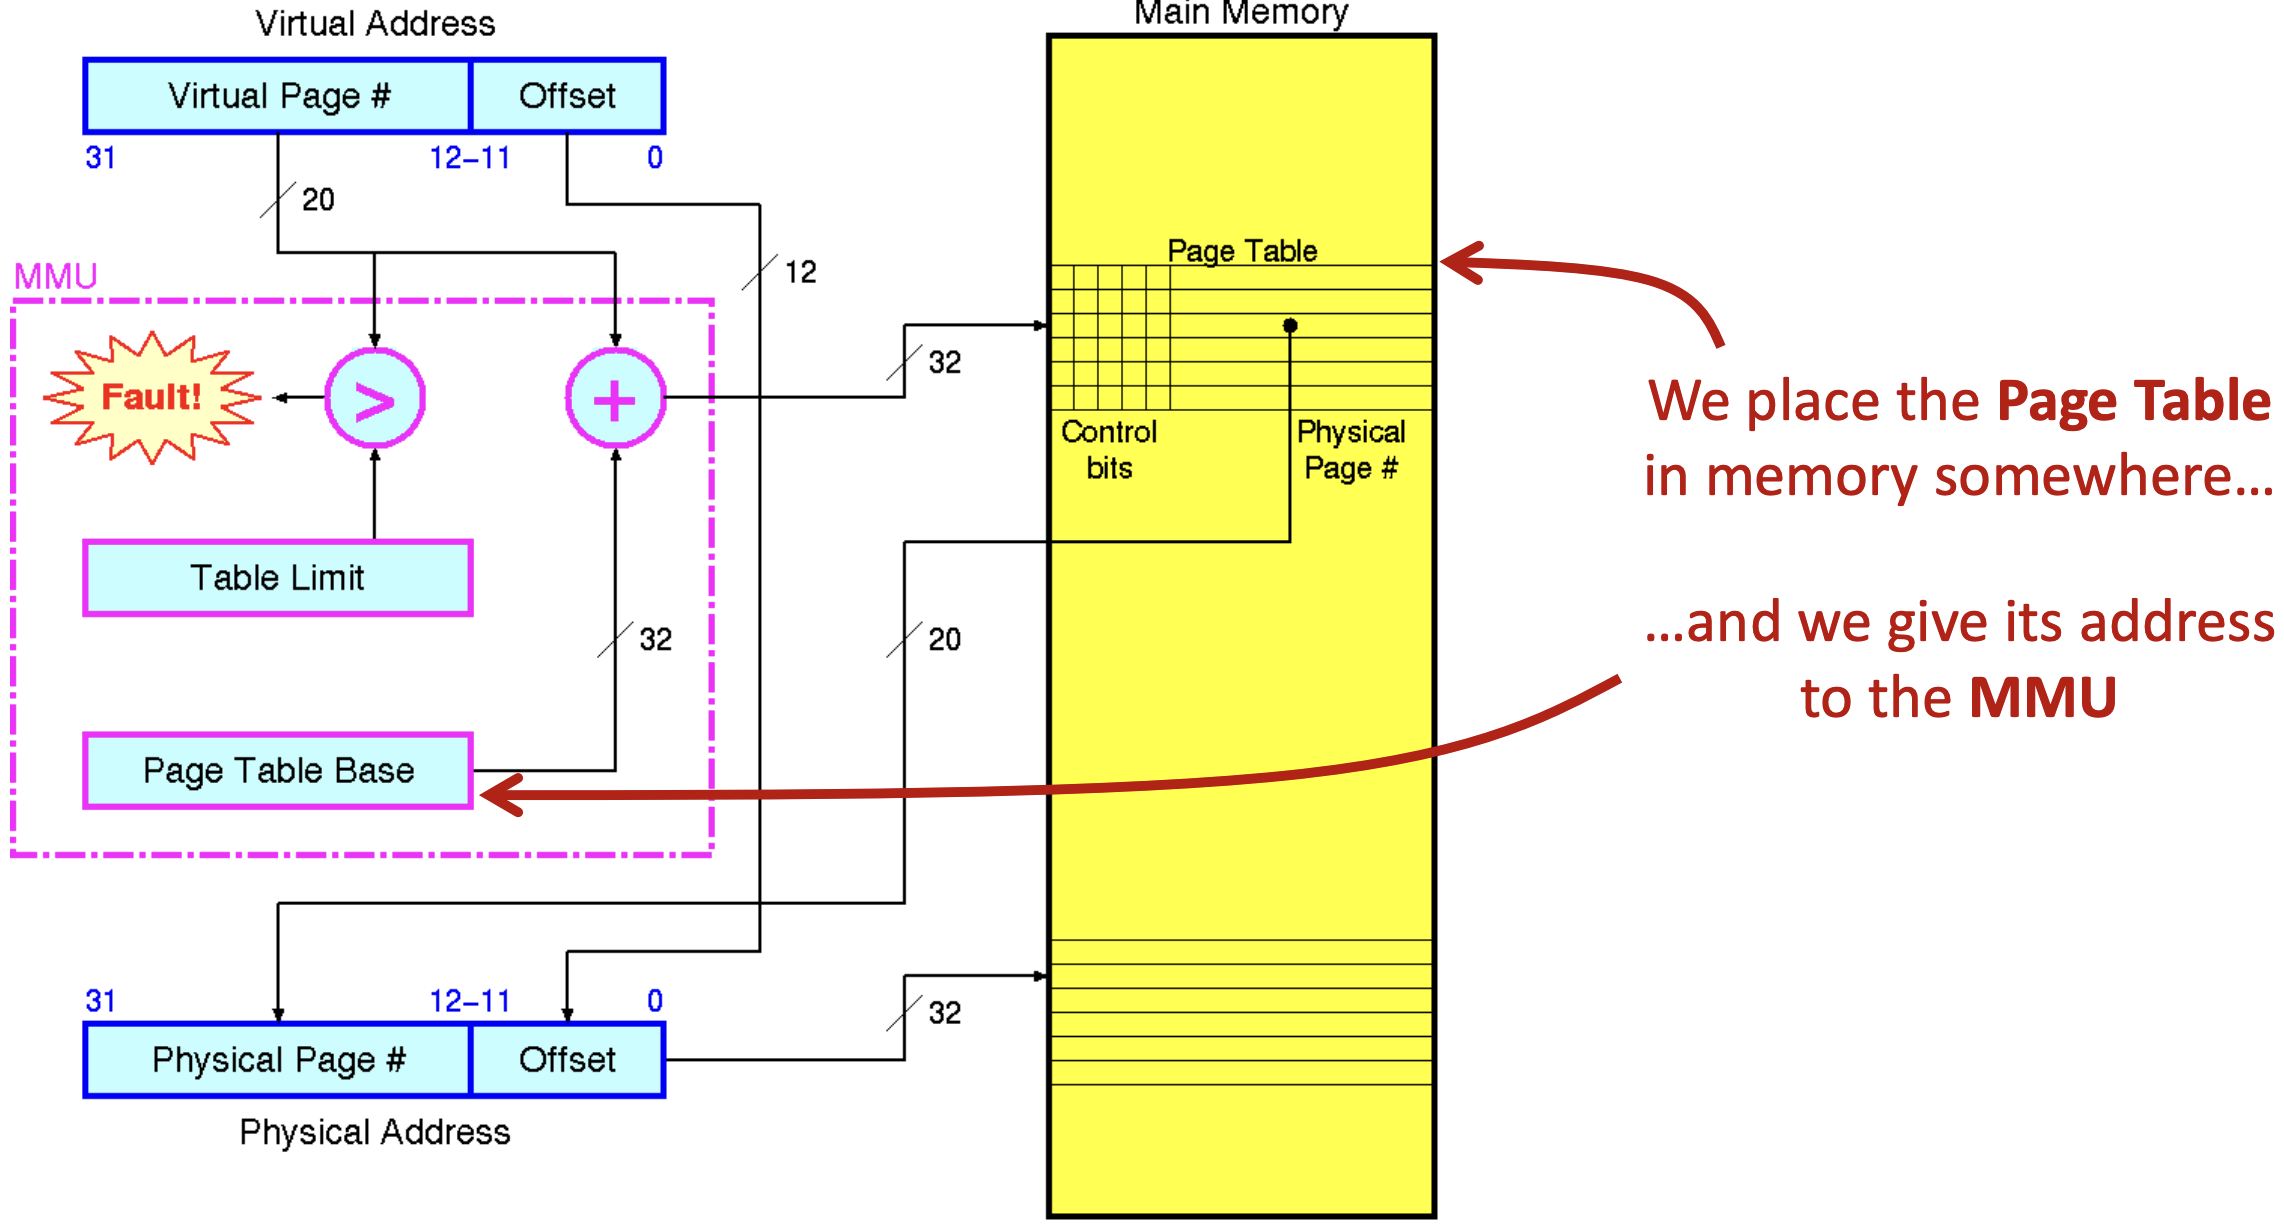
\includegraphics[width=0.65\textwidth]{chapters/chapter3c/images/pagedmmu.png}
\end{center}

\begin{itemize}
    \item[] \textbf{Page Table:}
    The page table, residing in main memory, contains:
    \begin{itemize}
        \item \textit{Control Bits:} Indicate the validity of a page and access permissions.
        \item \textit{Physical Page Numbers:} Map virtual pages to physical pages.
    \end{itemize}
\end{itemize}

\subsection{Memory Allocation is Easy Now}
Virtual memory systems simplify memory allocation by allowing noncontiguous physical memory to be mapped to contiguous virtual memory addresses. This enables efficient utilization of physical memory without requiring large, contiguous blocks.
\begin{center}
    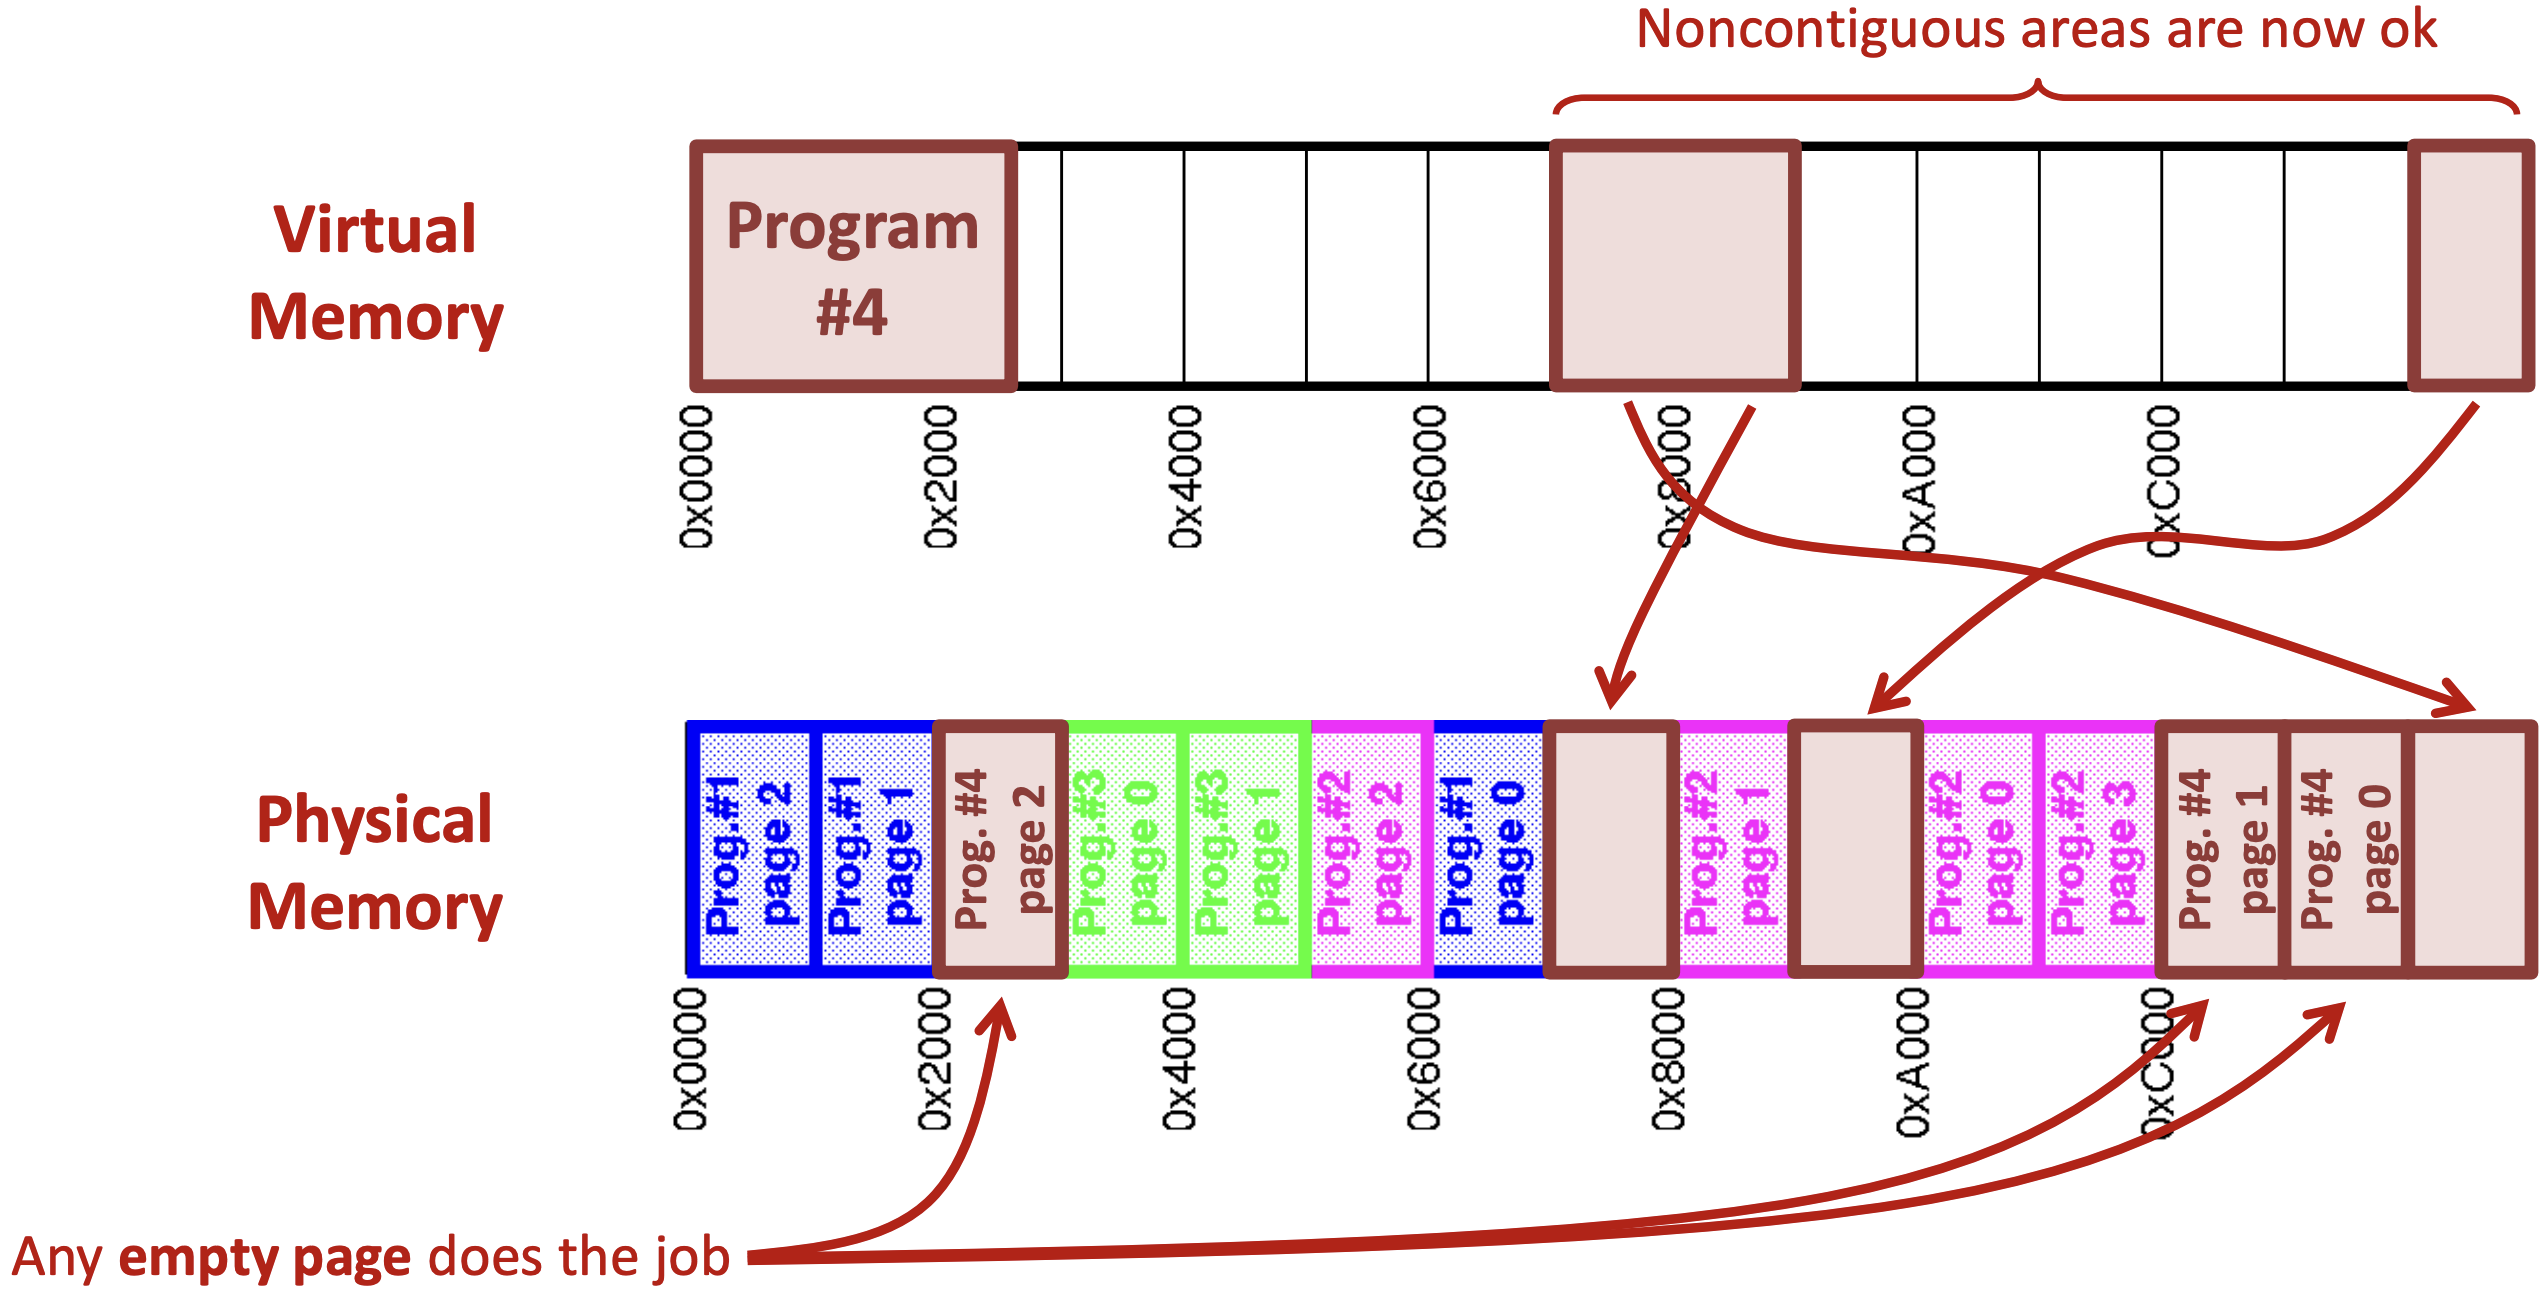
\includegraphics[width=0.65\textwidth]{chapters/chapter3c/images/relocation_bis.png}
\end{center}
\begin{itemize}
    \item[] \textbf{Virtual Memory:} Each program operates in its own virtual address space, making it unaware of the physical memory layout. Virtual addresses are mapped to physical addresses using a page table.
    \item[] \textbf{Physical Memory:} Physical memory is divided into fixed-size blocks called \textit{pages}. Any empty page in physical memory can be allocated to a program's virtual page.
    \item[] \textbf{Advantages:}
    \begin{itemize}
        \item Programs can use noncontiguous memory regions without manual intervention.
        \item Memory fragmentation is minimized since any available physical page can be used.
        \item Programs are isolated from one another, enhancing security and stability.
    \end{itemize}
    \item[] In the diagram above, Program \#4's virtual memory is mapped to noncontiguous pages in physical memory (e.g., 0x2000, 0x8000, and 0xC000). This flexibility ensures efficient allocation.
\end{itemize}

The use of virtual memory significantly enhances system performance and simplifies memory management by abstracting physical memory complexities.

\subsection{Page Tables and Their Size}
Page tables in virtual memory systems can grow significantly in size, especially in cases with large memory spaces. For instance, a memory size of 64 GiB with 4 KiB pages requires $2^{24}$ entries, amounting to approximately 64 MiB of space.

\textbf{Challenges} \\
For programs that utilize only a few megabytes, the majority of these entries remain empty, leading to inefficient memory usage.

\textbf{Solutions} \\
Several approaches exist to mitigate this inefficiency, including:
\begin{itemize}
    \item \textbf{Hashed Tables:} An alternative structure to reduce unused entries.
    \item \textbf{Paged Segmentation:} A hybrid approach to manage memory.
    \item \textbf{Multilevel Page Tables:} A hierarchical design to handle sparse page tables efficiently.
\end{itemize}

\subsection{Multilevel Page Tables}

Multilevel page tables are a hierarchical solution to reduce memory overhead caused by storing a single large page table. This structure is particularly useful in virtual memory systems with large address spaces.

\begin{center}
    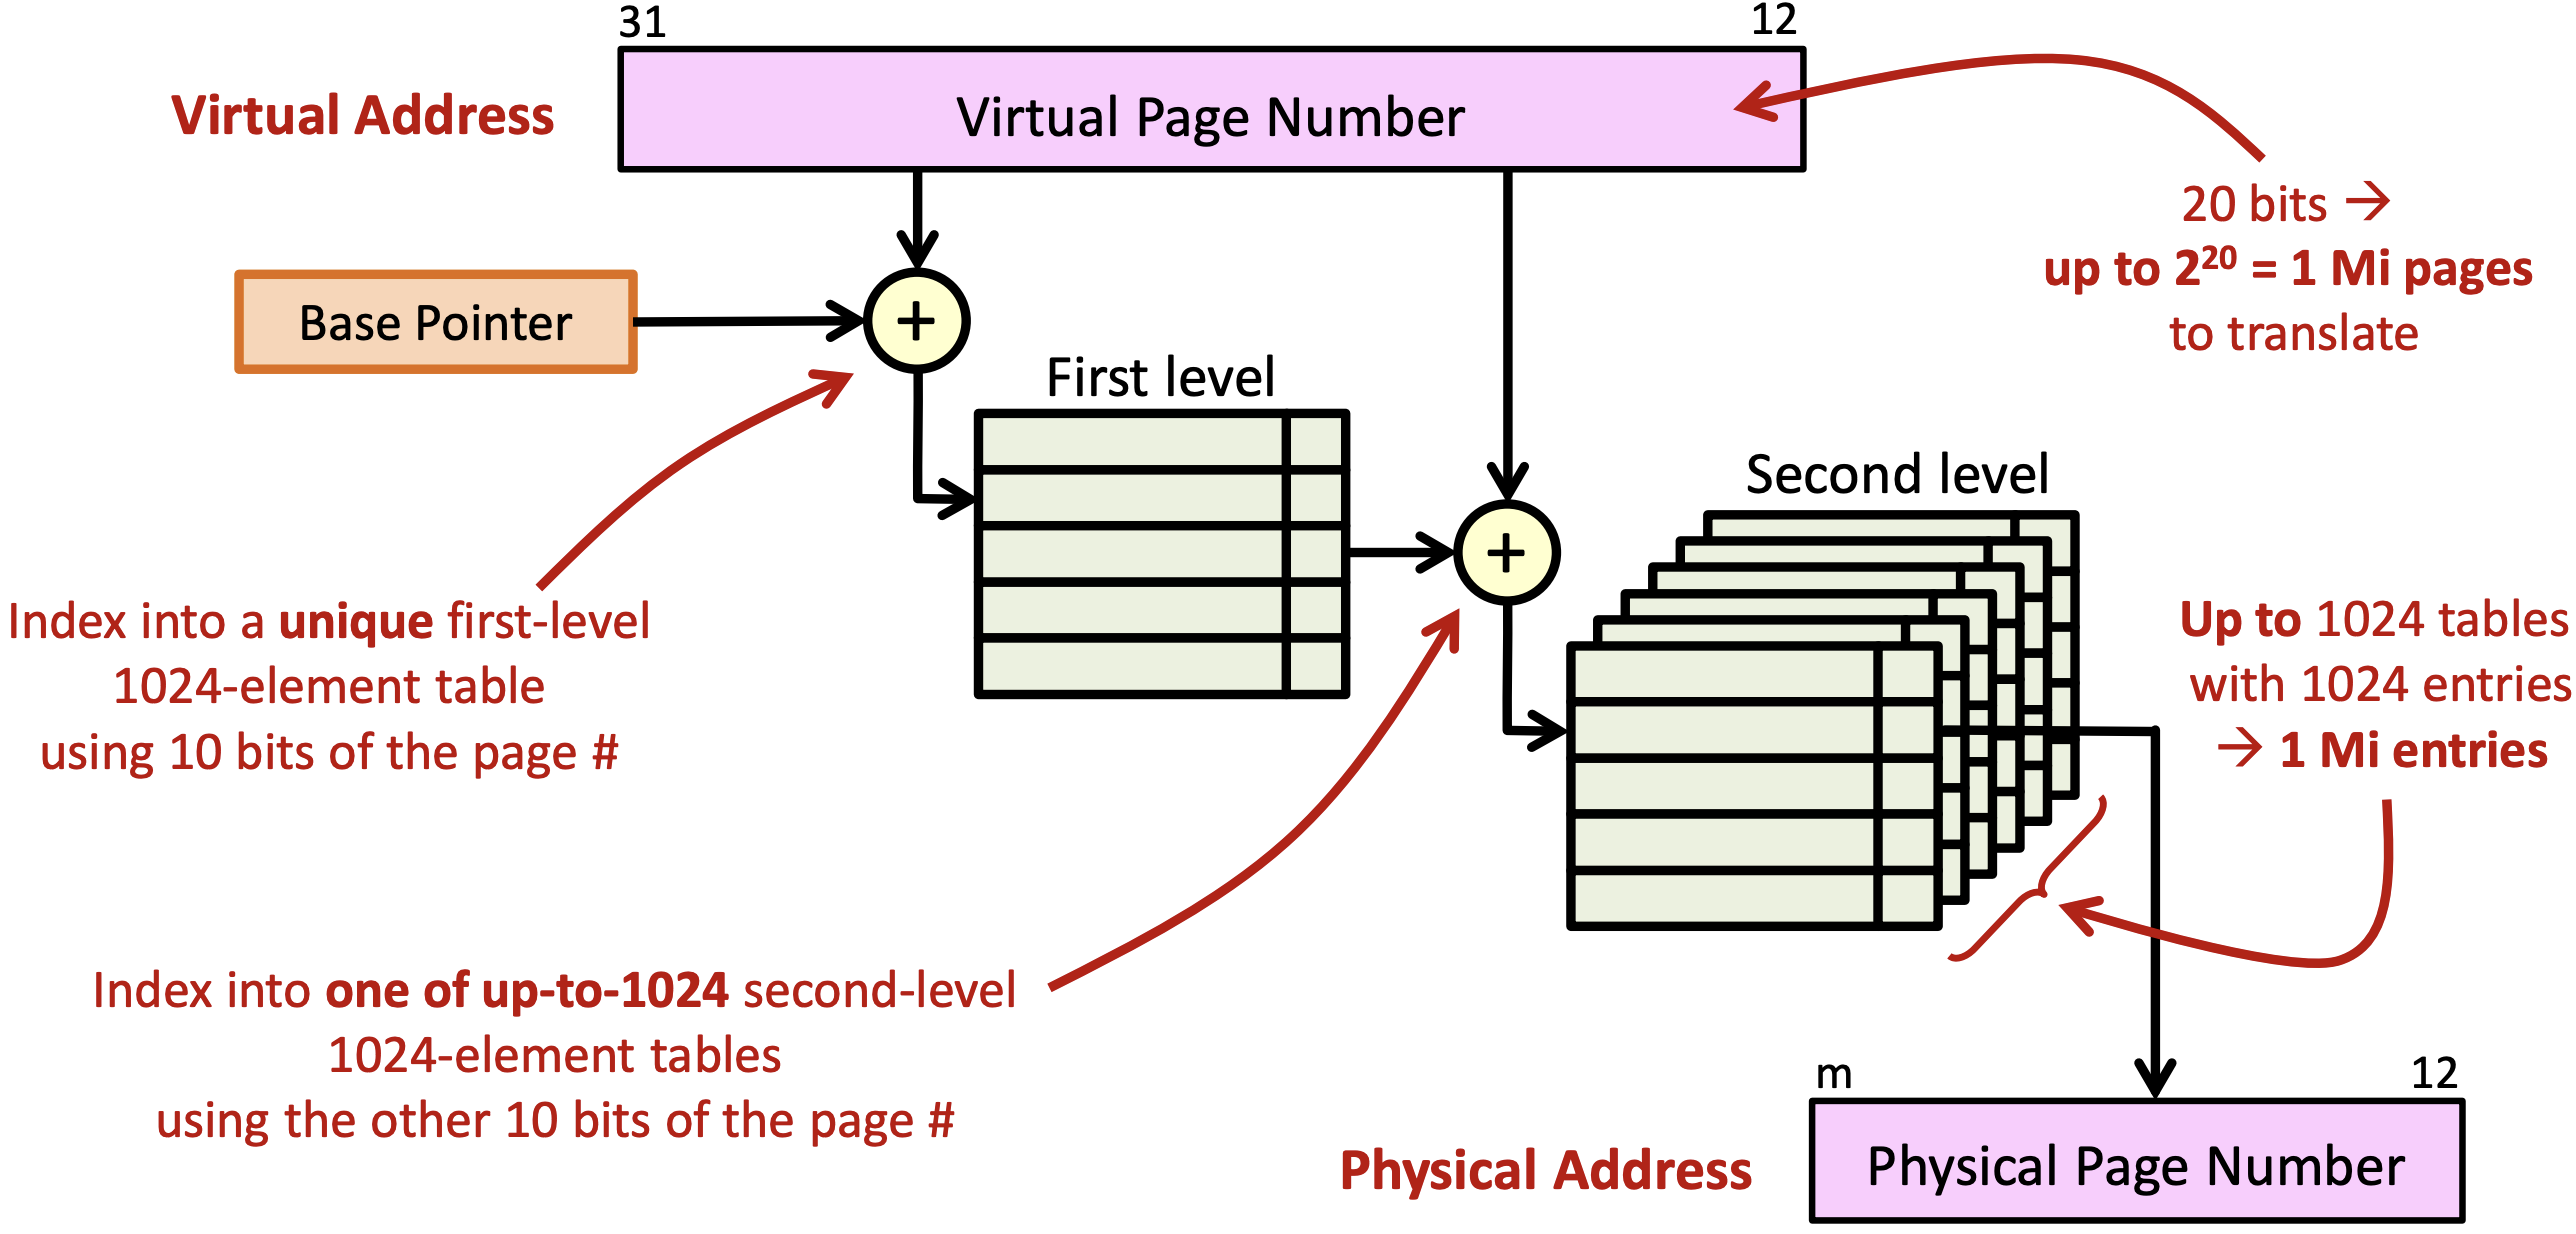
\includegraphics[width=0.65\textwidth]{chapters/chapter3c/images/multipage.png}
\end{center}
A virtual address is divided into three main parts:
\begin{itemize}
    \item \textbf{Virtual Page Number:} Determines the index within the page tables.
    \item \textbf{Page Offset:} Specifies the exact byte within the page.
\end{itemize}

The hierarchical organization involves:
\begin{enumerate}
    \item A \textbf{first-level page table}, indexed by the higher-order bits of the virtual page number. This table points to second-level page tables.
    \item \textbf{Second-level page tables}, indexed by the remaining bits of the virtual page number. These map to the physical page number.
\end{enumerate}

\textbf{Advantages:} \\
\begin{itemize}
    \item \textbf{Reduced memory usage:} Only necessary parts of the page tables are stored in memory.
    \item \textbf{Scalability:} Easily adapts to varying address space sizes.
\end{itemize}

\textbf{Key Steps in Address Translation:} \\
\begin{enumerate}
    \item Use the first-level index to locate the appropriate second-level page table.
    \item Use the second-level index to identify the physical page number.
    \item Combine the physical page number with the page offset to obtain the physical address.
\end{enumerate}

Multilevel page tables strike a balance between efficiency and memory overhead, making them a practical choice in modern operating systems.

